\chapter{Evaluation and Analysis}\label{chap:EvalAnalysis} 

In this chapter, we turn our attention to the evaluation and analysis of the randomized integration of the normalizing constant \(G_{\boldsymbol{\theta}}(\mathbf{N})\), via the Logistic Sampling algorithm, introduced in chapters 3 and 4. Since we are analyzing approximate, randomized, methods, special attention is paid to error analysis. More specifically, we are interested in the distribution of what will be random errors, and the factors that effect this distribution. The results from the experiments will be discussed along with their relations to theoretical properties.

\section{Overview of Experiments}\label{sec:overview_experiments}
The aim of this section is to give an overview of the scope of the experiments, and the general methodologies which will be employed. 
\\\\
The experiments will involve testing the integration methods of the integral form of the normalizing constants (\ref{eq:integral_form_single_server}), (\ref{eq:integral_form_infinite_server}), (\ref{eq:integral_form_multi_server_1}), and (\ref{eq:integral_form_multi_server_2}). These all involve using the Monte Carlo Integration via the Logistic Sampling Algorithm to integrate a uni-modal integrand \(e^{-f(\mathbf{x})}\) by summing:
\[I \approx \frac{1}{N} \sum_{i=1}^N \frac{e^{-f(\mathbf{x_i})}}{p(\mathbf{x_i})}\]
Where \(\mathbf{x_i}\) is drawn from some candidate sampling distribution with probability density function \(p(\mathbf{x})\).
\\\\
Since we are concerned with the behaviour of random errors on the computed value of the normalizing constant, it is important to be able to have a ground truth to test against. These will usually be calculated from an exact algorithm for smaller models \(G_{EXACT}\). Exact algorithms used as a baseline include the Recursion by Chain (RECAL) algorithm, the Method-of-Moments(MoM) and the Mean-Value-Analysis (MVA) algorithms. The choice of exact algorithms are primarily based on speed of computation, depending the size of the model. We are primarily interested in the normalizing constant \(G\), the queue-lengths \(Q_{kr}\) of the model, as well as the throughputs \(\lambda_{r}\). The errors for each metric are calculated:
\[E(G) = \frac{G_{LS} - G_{EXACT}}{G_{EXACT}}\]
\[E(Q) = \frac{\sum_{kr} |Q_{kr,LS} - Q_{kr,EXACT}|}{\sum_{kr} Q_{EXACT}}\]
\[E(\lambda) = \frac{\sum_{r} |\lambda_{r,LS} - \lambda_{r,EXACT}|}{\sum_{r} \lambda_{EXACT}}\]

For larger models, exact analysis becomes computationally intractable, and Logistic Sampling with a much larger (\(>3\) orders of magnitude) number of samples is used instead. The use of Logistic Sampling with over \(10^3\) times more samples should minimally impact the expected errors of solutions with a smaller number of samples, since the expected impact will be at least 30 times smaller than expected errors (the logistic sampling algorithm is tested with a maximum of \(10^4\) samples, and the approximated exact solution will be computed with \(10^7\) samples).
\\\\
Across all experiments, the default settings for the Logistic Sampling algorithm are used:
\begin{itemize}
    \item the additive logistic transformation for the integrand function
    \item the t-distribution with degree of freedom \(\nu=4\) for sampling distribution
\end{itemize}

The only exception to this rule is section \ref{sec:Transforms_and_Distributions} where a different transform and different sampling distributions are experimented with. 
\\\\
The experiments performed are summarized as below:
\begin{itemize}
    \item Sections \ref{sec:analyze_model_variation} - \ref{sec:Transforms_and_Distributions} will test single server models only. 
    \item Section \ref{sec:analyze_model_variation} will explore the effect of varying the demands \(\boldsymbol{\theta}\) of the model, as well as the population class share in the population vector \(\mathbf{N}\), for fixed total population \(N\).
    \item Section \ref{sec:Analyze_K_R_N} will analyze the effect of increasing the dimensionality of the integration domain by increasing the number of nodes in the system \(K\), as well as other hyper-parameters such as the number of classes \(R\), and total population \(N\).
    \item Section \ref{sec:Transforms_and_Distributions} will explore the effect of using different techniques to carrying out Monte Carlo Integration, namely by changing the type of logistic transform, and sampling distributions. 
    \item In section \ref{sec:Analyze_Delays} and \ref{sec:Multiserver}, the errors on different types of networks will be examined in relation to the single-server node networks. In the case of multi-server networks, special attention is paid to the phenomenon of variance cancellation.
\end{itemize}

\subsection{Interpretation of Errors}
Given that the Logistic Sampling Algorithm is in essence a randomized method, careful interpretation of the errors is required. Since the computed answers are random, it is important to think about error values not as a constant value, but as a random variable, with an associated distribution.
\\\\
\textit{{\large Mean Absolute Error and Uncertainties}}
\\\\
As a primary measure of error, we would like to evaluate the mean absolute percentage error (MAPE, denoted \(M\)) over a number of evaluations. This is calculated:
\begin{empheq}[box=\mymath]{equation}
    M = \frac{1}{N} \sum_{i=1}^N |\epsilon_i| 
\end{empheq}
Where \(\epsilon_i\) is the error calculated at an evaluation \(i\):
\[\epsilon_i = \frac{G_i-G_{i,EXACT}}{G_{i,EXACT}}\]

Where \(N\) is the number of evaluations. Given any distribution of \(\epsilon_i\), the central limit theorem (CLT) tells us that:
\[\bar{M} \sim \mathcal{N} \bigg(M, \frac{\sigma^2}{N} \bigg)\]
Where \(\bar{M}\) is the estimated mean of the distribution of absolute errors \(|\epsilon_i|\), and \(M\) and \(\sigma\) are the exact means and variances of this distribution. \(N\) is the number of evaluated errors.

In the case of unknown variance \(\sigma\), however, we can instead use the sample variance \(S^2\) of \(|\epsilon_i|\):
\[S^2 = \frac{1}{N} \sum_{i=1}^N (|\epsilon_i| - \bar{M})^2\]

Given that we can only estimate the variance, we can expect the true MAPE, \(M\), to be distributed according to a t-distribution with degree of freedom \(\nu=N-1\), mean \(\mu = \bar{M}\) and scale \(\sigma = \frac{S}{\sqrt{N}}\):
\begin{empheq}[box=\mymath]{equation}
    M \sim t_{n-1}\bigg(\bar{M}, \frac{S}{\sqrt{N}} \bigg)
\end{empheq}

This gives us an idea of the spread of the error distribution. This can also be useful when we would like to take confidences on the estimated MAPE. We will frequently show the plots of the MAPE with errorbars of 95\% confidence interval, as this can give us a better idea of the undelying error distribution.
\\\\
Besides that, having a probability distribution on the MAPE, \(M\) will allow us to perform some hypothesis testing, especially when comparing the relative effectiveness of different techniques with respect to the estimated errors.
\\\\
\textit{{\large Modelling the Error Distribution as a Normal Distribution}}
\\\\
Since the normalizing constant computed by the logistic integration can be interpreted as a mean of a function \(\frac{f(\mathbf{x})}{p(\mathbf{x})}\), sampled over \(p(\mathbf{x})\):
\[ G = E_{p\mathbf{(x)}} \bigg[ \frac{f(\mathbf{x})}{p\mathbf{(x)}} \bigg]\]
\[ \epsilon = \frac{G - G_{EXACT}}{G_{EXACT}} \]

The by CLT, the distribution of \(\epsilon\) should be normally distributed as \(N \rightarrow \infty\), given a model \( \mathcal{M} \) and number of samples \(N\).
\[ \epsilon_{|N,\mathcal{M}} \sim \mathcal{N}(0, \sigma_{|\mathcal{M}}(N))\]

Besides that, as has been explained in section \ref{sec:MCI}, the error is expected to be a linear function of the square root of \(N\):
\[\sigma_{|\mathcal{M}}(N) \propto N^{-1/2}\]

Therefore, we can expect that, given a fixed model \(\mathcal{M}\), the errors would be normally distributed.
\\\\
In several experiments, however, we would like to evaluate the distribution of the error with respect to some standard distribution, for a set of random models. The normal distribution is good to be used as a baseline to asses the symmetricity, and the relative spread of the error distribution, relative to the shape of the gaussian. To do this, for each experiment of a set of random models, we will fit a maximum-likelihood gaussian distribution to the set of errors:
\[\hat{\mu}_{ML} = \frac{1}{N} \sum_{i=1}^N \epsilon_i \quad \hat{\sigma}_{ML} = \frac{1}{N}\sum_{i=1}^N (\epsilon_i - \hat{\mu}_{ML})^2\]

The Kolmogorov-Smirnov (KS) statistic will be used as a goodness-of-fit score. When the KS score is low, this means that the normal approximation is a good one. A high KS score indicates large deviations from a normal distribution. 
 

\section{Analyzing the Effect of Model Variation}\label{sec:analyze_model_variation}

\subsection{Specific Models}\label{sec:experiments_specific_models}

Analysis of the effect of model variation began by looking at specific models, with deliberately chosen demands \(\boldsymbol{\theta}\). The methodology is as follows: 
\begin{itemize}[noitemsep]
    \item Size of the models were fixed, by fixing the number of stations \(K\), and the number of classes \(R\) to \(K=R=2\).
    \item The population vector \(\mathbf{N}\) was fixed to be \([3,3]\)
    \item The demands for station 0 was fixed to be \(\theta_{00} = \theta_{01} = 1.\)
    \item The demands for station 1 was changed according to the table \ref{tab:specific_models_evaluate}, to simulate different loads on the servers.
    \item The number of integration samples was fixed to \(N=100\).
    \item 300 evaluations were performed per model, and the errors calculated at each evaluation. The RECAL algorithm was used as ground truth.
\end{itemize}

\begin{table}[H]
\begin{center}
\begin{tabular}{@{}lllll@{}}
\toprule
 Test Case &  \(\theta_{10}\) & \(\theta_{11}\) & Description \\ \midrule
 1 & \(0.\) & \(0.\) & Load only on station 0 \\
 2 & \(0.25\) & \(0.25\) & Light load on station 1, heavy load on station 0\\
 3 & \(1.\) & \(1.\) & Perfectly equal loads \\
 4 & \(4.\) & \(4.\) & Symmetric model to case 1, with heavy load on station 1 \\ \bottomrule
\end{tabular}
\end{center}
\caption{Models tested}
\label{tab:specific_models_evaluate}
\end{table} 

For each model, the estimated mean absolute percentage error (MAPE), denoted \(\bar{M}\) and its 95\% confidence intervals was calculated:

\begin{table}[H]
\begin{center}
\begin{tabular}{@{}llllll@{}}
\toprule
 Test Case & \(\bar{M} \%\) & \(\bar{M}\) \(95\%\) CI (+) & \(\bar{M}\) \(95\%\) CI (-) & \(\hat{\sigma}_{ML}\)\\ \midrule
    1 &\(3.05\) & \(2.77\) & \(3.33\) & \(3.85\) &  \\ 
    2 &\(2.71\) & \(2.48\) & \(2.93\) & \(3.36\) &  \\ 
    3 &\(0.794\) & \(0.721\) & \(0.867\) & \(1.02\) &  \\ 
    4 &\(2.65\) & \(2.41\) & \(2.88\) & \(3.34\) &  \\  \bottomrule
\end{tabular}
\end{center}
\caption{Model errors}
\label{tab:specific_models_error}
\end{table} 

A surprising result was the difference in error distributions than can be seen between case 3 and the other test cases, where errors were much lower than in the other cases. A quick look at the error histograms confirm this finding to be true. Besides that, the QQ plots show good conformity of the error distribution with its maximum likelihood normal distributions.

\begin{figure}[!htb]
\begin{center}
    \centering
    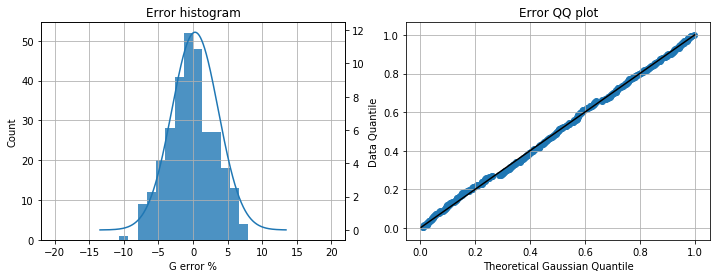
\includegraphics[width=1.0\textwidth]{Chap6_EvaluationAndAnalysis/images/Error_model_D_1_1_025_025_N_3_3.png}
\caption{Error distribution (fitted ML Gaussian in blue line) and QQ plot for case 2 -  \(\theta_{10}=\theta_{11}=0.25\)}
\label{fig:error_model_D_1_1_025_025_N_3_3}
\end{center}
\end{figure}

\begin{figure}[!htb]
\begin{center}
    \centering
    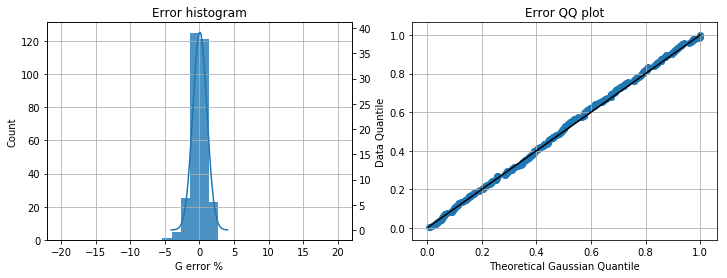
\includegraphics[width=1.0\textwidth]{Chap6_EvaluationAndAnalysis/images/Error_model_D_1_1_1_1_N_3_3.png}
\caption{Error distribution and QQ plot for case 3 - \(\theta_{10}=\theta_{11}=1\)}
\label{fig:error_model_D_1_1_1_1_N_3_3}
\end{center}
\end{figure}

When inspecting the shape of the integrand, one feature stood out for case 3 against all the remaining cases. The integrand was symmetric about its stationary point, as can be seen by comparing figure \ref{fig:spec_model_D_1_1_1_1_N_3_3} against figures \ref{fig:spec_model_D_1_1_0_0_N_3_3}, and \ref{fig:spec_model_D_1_1_4_4_N_3_3}.

\begin{figure}[!htb]
\begin{center}
\begin{subfigure}%[Simplex]
    \centering
    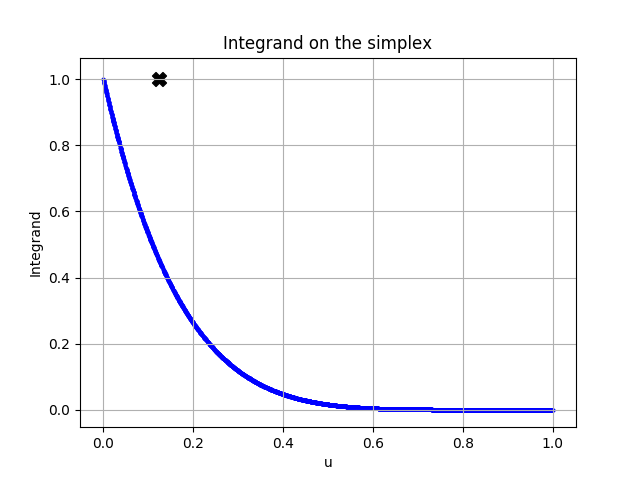
\includegraphics[height=2in]{Chap6_EvaluationAndAnalysis/images/Simplex_model_D_1_1_0_0_N_3_3.png}
\end{subfigure}
\begin{subfigure}%[Real]
    \centering
    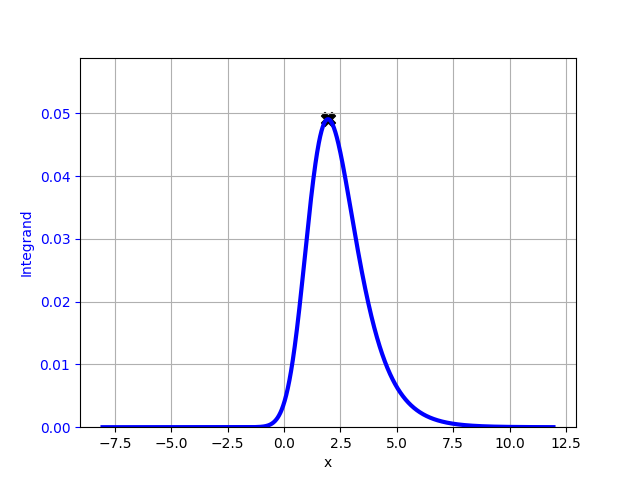
\includegraphics[height=2in]{Chap6_EvaluationAndAnalysis/images/Real_model_D_1_1_0_0_N_3_3.png}
\end{subfigure}
\caption{Test case 1 - \(\theta_{10}=\theta_{11}=0\). (Left) Shape of integrand on the simplex (Right) Shape of integrand after transform. Black cross in right plot represents stationary point of integrand function, and is re-projected back onto the simplex, shown in the left plot.}
\label{fig:spec_model_D_1_1_0_0_N_3_3}
\end{center}
\end{figure}

\begin{figure}[!htb]
\begin{center}
\begin{subfigure}%[Simplex]
    \centering
    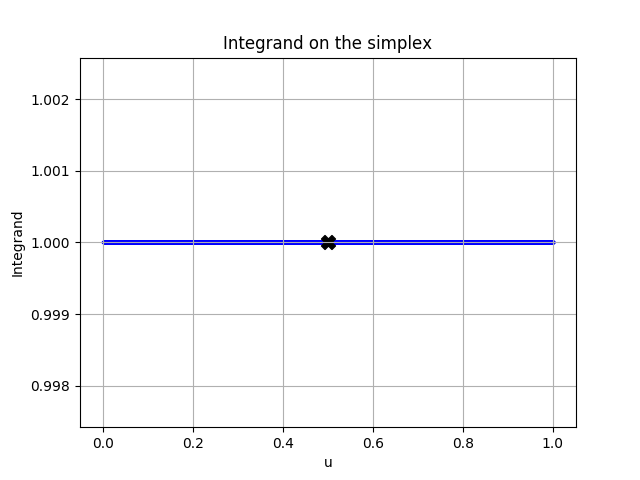
\includegraphics[height=2in]{Chap6_EvaluationAndAnalysis/images/Simplex_model_D_1_1_1_1_N_3_3.png}
\end{subfigure}
\begin{subfigure}%[Real]
    \centering
    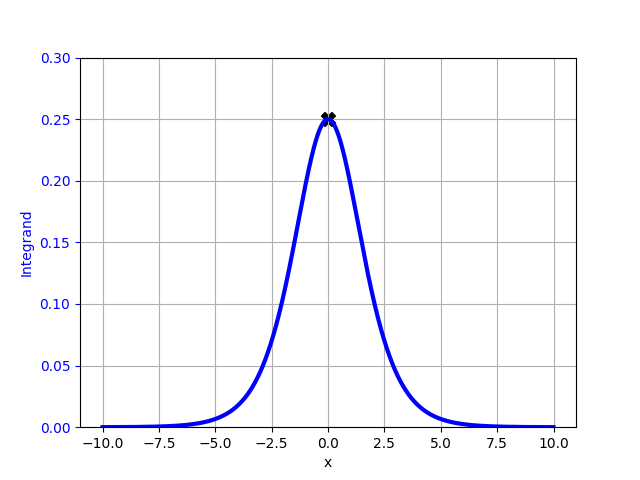
\includegraphics[height=2in]{Chap6_EvaluationAndAnalysis/images/Real_model_D_1_1_1_1_N_3_3.png}
\end{subfigure}
\caption{Test case 2 - \(\theta_{10}=\theta_{11}=1\)}
\label{fig:spec_model_D_1_1_1_1_N_3_3}
\end{center}
\end{figure}

 We can also inspect the shape of the distribution with respect to the integrand by overlaying the plot of the sampling distribution PDF of the model, and of the function to be integrated. It can be seen that the shape of the distribution in figure \ref{fig:sampling_pdfs_model}, for the left plot representing test case 2, the sampling distribution conforms much better with the integrand, while on the right plot which represents test case 3, the sampling distribution cannot capture the skewness of the integrand function. As discussed in section \ref{sec:MCI}, this would affect the contribution of the \(\frac{f(\mathbf{x})}{p(\mathbf{x})}\) term to the variance of the estimated integral \(\widetilde{I}\), and potentially lower the efficiency of the sampling. 
 
\begin{figure}[!htb]
\begin{center}
\begin{subfigure}%[Simplex]
    \centering
    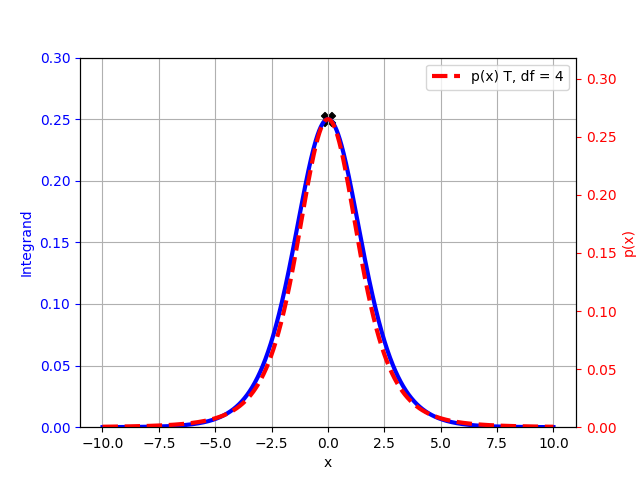
\includegraphics[height=2in]{Chap6_EvaluationAndAnalysis/images/px_D_1_1_1_1_N_3_3.png}
\end{subfigure}
\begin{subfigure}%[Real]
    \centering
    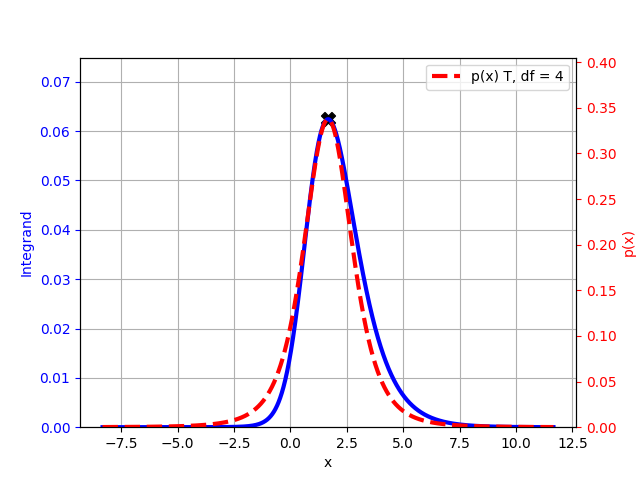
\includegraphics[height=2in]{Chap6_EvaluationAndAnalysis/images/px_D_1_1_025_025_N_3_3.png}
\end{subfigure}
\caption{Integrand (blue) overlaid with sampling distribution (red): Test Case 2 (Left) \(\theta_{10}=\theta_{11}=1\), Test Case 3 (Right) \(\theta_{10}=\theta_{11}=0.25\)}
\label{fig:sampling_pdfs_model}
\end{center}
\end{figure}

\begin{figure}[!htb]
\begin{center}
\begin{subfigure}%[Simplex]
    \centering
    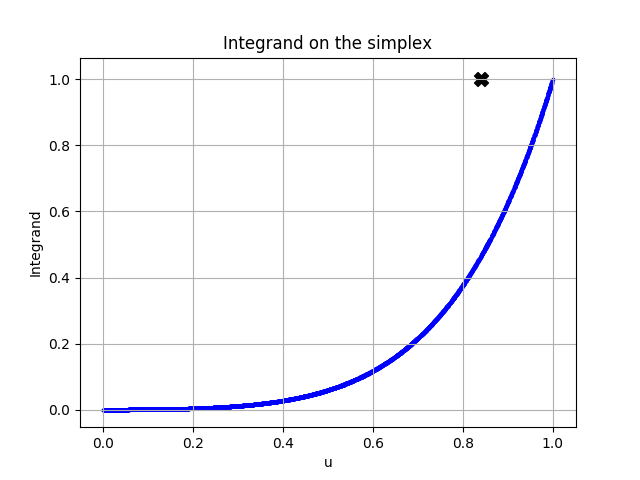
\includegraphics[height=2in]{Chap6_EvaluationAndAnalysis/images/Simplex_model_D_1_1_4_4_N_3_3.png}
\end{subfigure}
\begin{subfigure}%[Real]
    \centering
    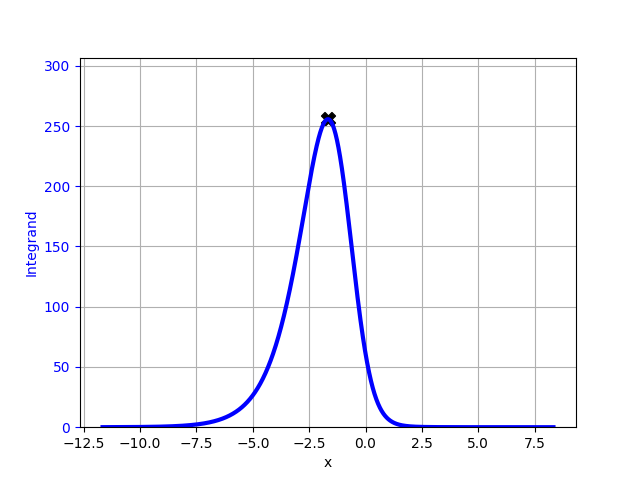
\includegraphics[height=2in]{Chap6_EvaluationAndAnalysis/images/Real_model_D_1_1_4_4_N_3_3.png}
\end{subfigure}
\begin{subfigure}%[Simplex]
    \centering
    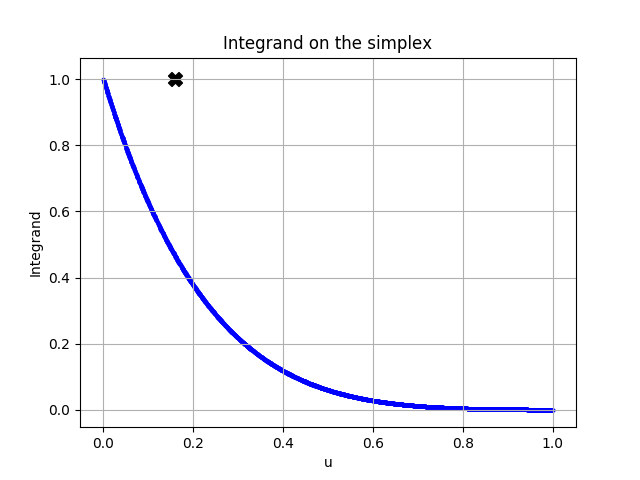
\includegraphics[height=2in]{Chap6_EvaluationAndAnalysis/images/Simplex_model_D_1_1_025_025_N_3_3.png}
\end{subfigure}
\begin{subfigure}%[Real]
    \centering
    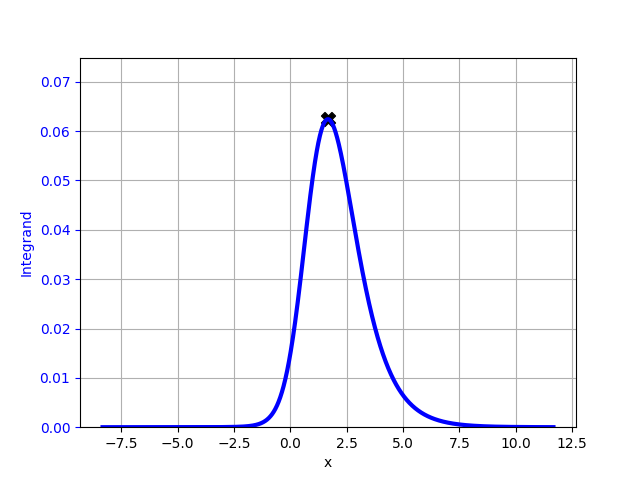
\includegraphics[height=2in]{Chap6_EvaluationAndAnalysis/images/Real_model_D_1_1_025_025_N_3_3.png}
\end{subfigure}
\caption{Test case 3 - (top) \(\theta_{10}=\theta_{11}=0.25\), Test case 4 - (bottom) \(\theta_{10}=\theta_{11}=4\)}
\label{fig:spec_model_D_1_1_4_4_N_3_3}
\end{center}
\end{figure}

\subsection{Relating Stationary Point Location with Expected Errors}

It was believed that one source of the skewness observed in the previous section's test cases was due to the location of the stationary point in the simplex. The shape of functions with skewed stationary points tend to more skewed on the simplex, this is also further magnified by the effect of the Jacobian which is a concave function on the simplex, and introduces a sharper gradient on the function about its stationary point, for skewed stationary points on the simplex, giving it asymmetry.
\\\\
In order to investigate this, a similar experiment to the one in section \ref{sec:experiments_specific_models} was performed. However, instead of hand-picking 4 models to evaluate, \(60 \times 60\) models were evaluated. Models with \(K=R=2\) were tested. \(60\) evenly spaced values each of \(\theta_{10}\) and \(\theta_{11}\), between \(\theta=0.0\) and \(\theta=4.0\). At each value of the \((\theta_{10}, \theta_{11})\) pair, 20 evaluations of the normalizing constant were performed, and a MAPE value was calculated.
\\\\
3 experiments were conducted with the above setup. In each experiment, the population vector was changed. For \(N=6\), 3 population shares were investigated: \(\mathbf{N} = [3,3]\), \(\mathbf{N} = [2,4]\), \(\mathbf{N} = [1,5]\). 
\\\\
Since we are trying to find out if stationary point deviation from the centre of the simplex affects the error of the model calculation, we seek to identify models with stationary points satisfying the following relation (where \(\mathbf{\hat{u}}\) is the stationary point of the model):
\[\hat{u}_0 = \hat{u}_1 = ... = \hat{u}_K = 1/K\]

For the 2 station case (\(K=2\)), given a population vector \(\mathbf{N} = [N_0, N_1]\), the stationary point equations become (for \(i = 1,2\)):
\[0.5 = \eta^{-1}(N) \bigg( 1 + 0.5 \sum_{r=1}^R \xi_r(\mathbf{\hat{u}}) \theta_{ir} \bigg)\]
Where \( \xi_r(\mathbf{\hat{u}}) = 0.5 N_r (\sum_{k=1}^K \theta_{kr})\)
\\\\
In all three experiments, demands for station 1 was set to 1. for all classes \(\theta_{00} = \theta_{01} = 1.\) The system of equations reduces to:
\[ \theta_{00} \xi_0 + \theta_{01} \xi_1 = \theta_{10} \xi_0 + \theta_{11} \xi_1\]

Using the definition of \(\xi_0, \xi_1\) and the fact that \(\theta_{00} = \theta_{01} = 1.\), the equation reduces to:
\begin{empheq}[box=\mymath]{equation}
    \label{eq:centre of simplex models}
    \frac{N_0}{1 + \theta_{10}} + \frac{N_1}{1 + \theta_{11}} = \frac{N_0 \theta_{10}}{1 + \theta_{10}} + \frac{N_1 \theta_{11}}{1 + \theta_{11}}
\end{empheq}
Therefore, the models of interest have \(\theta_{10}\) and \(\theta_{11}\) which satisfy the above equation.
\\\\
\textit{{\large Test Case 1: \(\mathbf{N} = [3,3]\)}}\\
In the first case, the population vector was set to \((3,3)\). When \(N_0 = N_1 = N\), the equation (\ref{eq:centre of simplex models}) simplifies to become:
\begin{empheq}[box=\mymathtwo]{equation*}
    \theta_{10} = \frac{1}{\theta_{11}}
\end{empheq}


The color in figure \ref{fig:bottleneck_analysis_balanced_pop} shows the distribution of errors, with the color scale shown on the right. The region of lowest error corresponds to the region around the line \(y = 1/x\), which represent models having stationary points at the centre of the simplex. \\

\begin{figure}[!htb]
\begin{center}
    \centering
    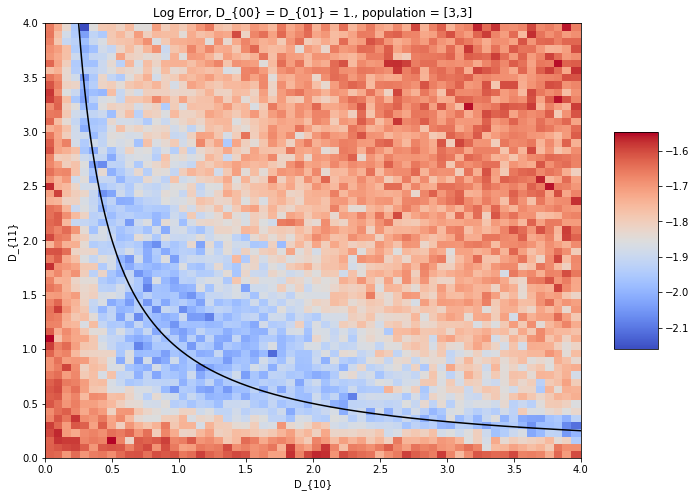
\includegraphics[width=0.8\textwidth]{Chap6_EvaluationAndAnalysis/images/error_analysis_bottleneck_balanced_pop.png}
\caption{Error plot for models and population \(\mathbf{N}=[3,3]\)}
\label{fig:bottleneck_analysis_balanced_pop}
\end{center}
\end{figure}

This does not seem to have any relation with the notion of a 'bottleneck' station. For the above model with the specified population, the line of constant load for station 1 is: 
\[\theta_{10} + \theta_{11} = C\]

Where \(C\) is a constant denoting the relative load on the second station. When \(C=2\), the load is balanced between station 0 and station 1. When \(C>2\), station 1 is more heavily loaded, and when \(C<2\), station 0 is more heavily loaded. However, it can be seen that lines of constant \(C\) to not correspond to lines of constant error. 
\\\\
\textit{{\large Test Case 2: \(\mathbf{N} = [2,4]\)}}
\\
The error color plot for this is shown in figure \ref{fig:bottleneck_analysis_pop_24}. When the population vector is set to \(\mathbf{N} = [2,4]\), the centre-of-simplex equations becomes:
\begin{empheq}[box=\mymathtwo]{equation*} \theta_{11}(3 \theta_{10} - 1) = 3 - \theta_{10} \end{empheq}
Again, the line of minimum error \(y = (3 - x)/(3x - 1)\) is plotted in black against the error color plot.\\\\

\begin{figure}[!htb]
\begin{center}
    \centering
    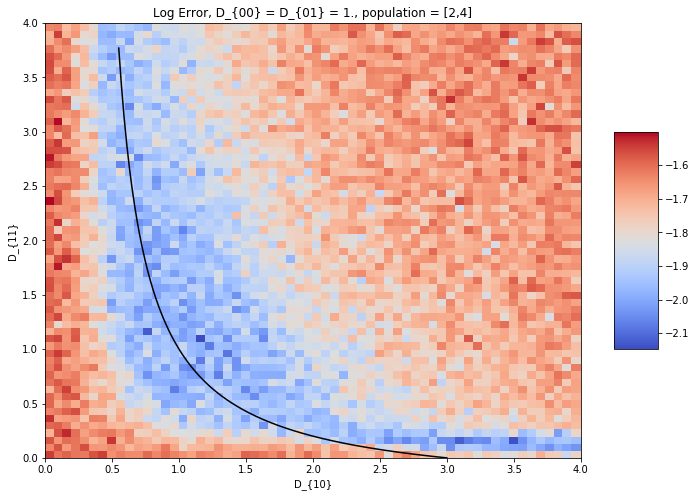
\includegraphics[width=0.8\textwidth]{Chap6_EvaluationAndAnalysis/images/error_analysis_bottleneck_pop_24.png}
\caption{Error plot for models and population \(\mathbf{N}=[2,4]\)}
\label{fig:bottleneck_analysis_pop_24}
\end{center}
\end{figure}

\textit{{\large Test Case 3: \(\mathbf{N} = [5,1]\)}}\\

\begin{figure}[!htb]
\begin{center}
    \centering
    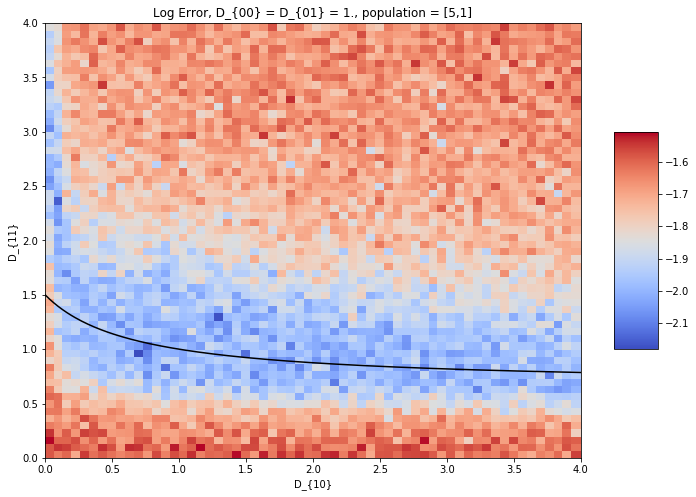
\includegraphics[width=0.8\textwidth]{Chap6_EvaluationAndAnalysis/images/error_analysis_bottleneck_pop_51.png}
\caption{Error plot for models and population \(\mathbf{N}=[5,1]\)}
\label{fig:bottleneck_analysis_pop_51}
\end{center}
\end{figure}

The error color plot for this is shown in figure \ref{fig:bottleneck_analysis_pop_51}. When the population vector is set to \(\mathbf{N} = [5,1]\), equation \ref{eq:centre of simplex models} becomes:
\begin{empheq}[box=\mymathtwo]{equation*} \theta_{11}(3 \theta_{10} + 2) = 3 + 2 \theta_{10} \end{empheq}
This gives us the black line of minimum error as shown in figure \ref{fig:bottleneck_analysis_pop_51}. 
\\\\
It is also quite interesting to plot the MAPE of the normalizing constant estimate, against distance of a model's stationary point from the centre of a simplex. The plot in figure \ref{fig:MAPE_vs_uhat} shows good correlation between the two quantities.
\begin{figure}[!htb]
\begin{center}
    \centering
    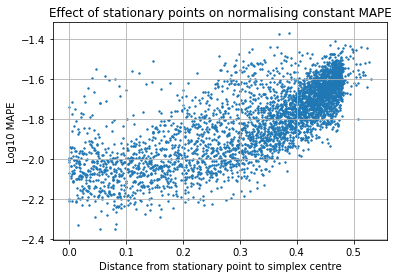
\includegraphics[width=0.8\textwidth]{Chap6_EvaluationAndAnalysis/images/NC_error_vs_uhat.png}
\caption{Plot of \(\log_{10}(MAPE)\) against distance of \(\mathbf{\hat{u}}\) from centre of simplex}
\label{fig:MAPE_vs_uhat}
\end{center}
\end{figure}

In conclusion, in general, there does not seem to be any correlation with the physical notion of the 'loading' of certain stations, and calculation errors of the normalizing constant. The shape of the integrand has a much larger part to play in the error estimate of the model, since this is a dominating factor in the efficiency of Monte Carlo Sampling, and by extension the Logistic Sampling algorithm. Although by no means a strict rule, it seems to be the general trend that a well-centered model on the simplex tends to be more accurately calculated. These are models which satisfy the following equation:

\[K^{-1} = \eta^{-1}(N) \bigg( 1 + \sum_{r=1}^R \frac{N_r \theta_{ir}}{\sum_k^K \theta_{kr} } \bigg)\]

\section{Effects of Number of Classes, Servers, and Populations}\label{sec:Analyze_K_R_N}
In this section, we will try to analyze the error distribution with respect to the size of the model. We begin first by looking at the convergence behaviour of errors with respect to the number of integration samples \(n_s\). Next we will observe the behaviour of errors with respect to number of classes, population, and finally the number of stations.
\\\\
Two experiments were conducted for the error analysis: 
\begin{itemize}[noitemsep]
    \item A set of small models where \(K,R \in [2,4,6]\) , and a set of medium-large models where \(K,R \in [8,12,16]\) were tested.
    \item For each combination of \(K\) and \(R\), 100 randomized models were tested, where \(\theta\) was sampled uniformly. Hence the effect of a model \(\mathcal{M}\) was marginalized out.
    \item For each model the population was ramndomized, where each class population \(N_r \sim \mathcal{U}(1,5)\). 
    \item Each model was tested with a different number of samples, ranging from \(10^1\) to \(10^4\).
\end{itemize}

\subsection{Initial look at Convergence}
An initial look at the convergence plots for small models (\(K,R \in [2,4,6]\)) shows that Monte Carlo Integration theory is right: that the estimated error is square-root convergent. The tabulated errors in table \ref{tab:convergence_tabulated_errors} show the MAPE for the normalizing constant (denoted \(\bar{M}(G)\)), the queue-lengths (\(\bar{M}(Q)\)) and throughputs (\(\bar{M}(\lambda)\)), averaged over all \(3 \times 3 \times 100\) models. The max-likelihood estimate of the \(G\) standard error is denoted \(\hat{\sigma}(G)\). The KS score is also shown, indicating slight deviation from normality, given that a variety of models of different sizes are considered.
\\\\
Furthermore, figure \ref{fig:OverallConvergence} on the right plots the log (base 10) of estimated MAPE values against the number of samples on a log scale. The gradients of these plots can be seen to be almost exactly \(1/2\). These values are again plotted on the right figure \ref{fig:OverallConvergence} alongside errorbars representing the 95\% confidence interval of the true value of the MAPE. The MAPE for Queue Length and Throughputs can be seen to be slightly higher on average since they involve computing more than 1 value of a normalizing constant.

\begin{table}[H] 
\begin{center}
\begin{tabular}{@{}lllllll@{}}
\toprule
    \(N\) & KS score & \(\bar{M}(G)\) \% & \(\hat{\sigma}(G)\) \% & \(\bar{M}(Q)\) \% & \(\bar{M}(\lambda)\) \% \\  \midrule
    10 &\(0.091\) & \(14.979\) & \(20.834\) & \(26.782\) & \(22.251\) &  \\ 
    20 &\(0.115\) & \(11.413\) & \(17.019\) & \(18.079\) & \(16.251\) &  \\ 
    50 &\(0.102\) & \(6.948\) & \(10.214\) & \(11.713\) & \(9.717\) &  \\ 
    100 &\(0.098\) & \(5.077\) & \(7.300\) & \(8.515\) & \(7.123\) &  \\ 
    200 &\(0.093\) & \(3.636\) & \(5.239\) & \(6.395\) & \(5.185\) &  \\ 
    500 &\(0.096\) & \(2.272\) & \(3.241\) & \(3.942\) & \(3.322\) &  \\ 
    1000 &\(0.095\) & \(1.743\) & \(2.507\) & \(2.759\) & \(2.478\) &  \\ 
    2000 &\(0.086\) & \(1.198\) & \(1.693\) & \(1.940\) & \(1.690\) &  \\ 
    5000 &\(0.085\) & \(0.782\) & \(1.120\) & \(1.255\) & \(1.075\) &  \\ 
    10000 &\(0.080\) & \(0.526\) & \(0.751\) & \(0.860\) & \(0.745\) &  \\     \bottomrule
\end{tabular}
\end{center}
\caption{Tabulated Mean Absolute Percentage Error(MAPE, denoted \(E\)) and standard errors denoted \(\sigma\), for small models \(K,R \in [2,4,6]\)}
\label{tab:convergence_tabulated_errors}
\end{table} 

\begin{figure}[!htb]
\begin{center}
\begin{subfigure}
    \centering
    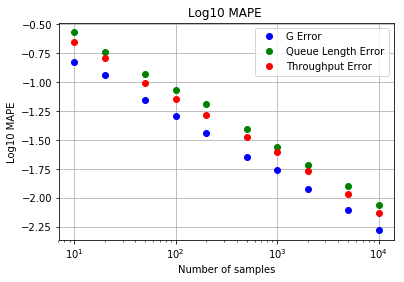
\includegraphics[width=0.45\textwidth]{Chap6_EvaluationAndAnalysis/images/OverallConvergence.png}
\end{subfigure}
\begin{subfigure}
    \centering
    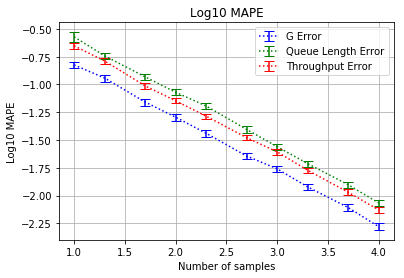
\includegraphics[width=0.45\textwidth]{Chap6_EvaluationAndAnalysis/images/OverallConvergenceSigma.png}
\end{subfigure}
\caption{(Left) Convergence plot for log10 MAPE, (Right) with 95\% CI errorbars}
\label{fig:OverallConvergence}
\end{center}
\end{figure}

\begin{figure}[!htb]
\begin{center}
    \centering
    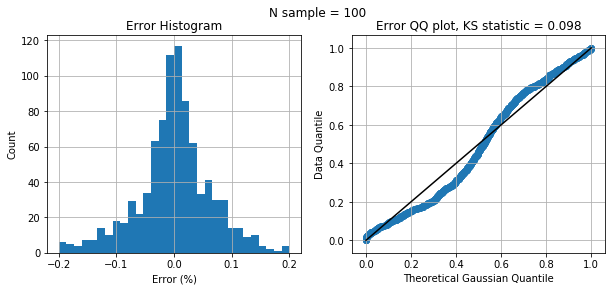
\includegraphics[width=0.8\textwidth]{Chap6_EvaluationAndAnalysis/images/N100_KR246.png}    
\caption{Error histogram (Left) and QQ plot (Right) of the errors vs. its Max Likelihood Gaussian for all small models (\(K,R \in [2,4,6]\)), and number of smaples = \(100\), shown with its Kolmogorov-Smirnov statistic. Both the KS statistic and QQ plots indicate slight divergence from normality}
\label{fig:ErrorHistN100_KR246}
\end{center}
\end{figure}

\subsection{Varying model size and population}

Separating the datasets by number of classes and plotting a convergence plot, we see quite clearly that the error distribution for the models hardly depends on the number of classes of customers in the model. This is a very good property to have, since we can scale the number of classes in the model up, without having to worry about increasing errors.

\begin{figure}[!htb]
\begin{center}
\begin{subfigure}
    \centering
    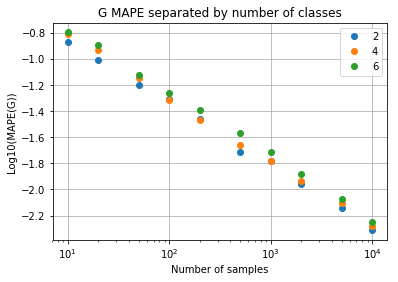
\includegraphics[width=0.45\textwidth]{Chap6_EvaluationAndAnalysis/images/ConvergenceNumberOfClasses_SM_meanerr.png}
\end{subfigure}
\begin{subfigure}
    \centering
    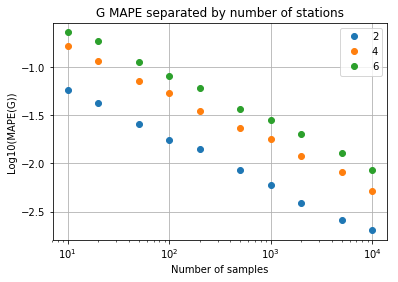
\includegraphics[width=0.45\textwidth]{Chap6_EvaluationAndAnalysis/images/ConvergenceNumberOfStations_SM_meanerr.png}
\end{subfigure}
\caption{Convergence plot for the MAPE of normalizing constant \(\bar{M}(G)\), separated by number of classes (left) ,and number of stations (right)}
\label{fig:ClassSeparatedConvergence_MAPE}
\end{center}
\end{figure}

\begin{figure}[!htb]
\begin{center}
\begin{subfigure}
    \centering
    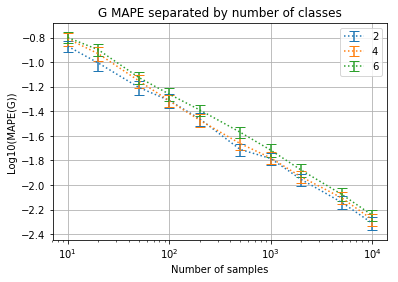
\includegraphics[width=0.45\textwidth]{Chap6_EvaluationAndAnalysis/images/ConvergenceNumberOfClasses_SM.png}
\end{subfigure}
\begin{subfigure}
    \centering
    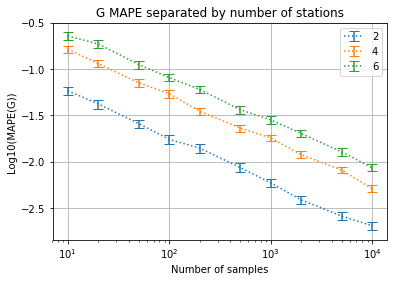
\includegraphics[width=0.45\textwidth]{Chap6_EvaluationAndAnalysis/images/ConvergenceNumberOfStations_SM.png}
\end{subfigure}
\caption{Convergence plot for the MAPE of normalizing constant \(\bar{M}(G)\) for small models, errorbars are \(95\%\) CI from t-distribution of the true MAPE}
\label{fig:ClassSeparatedConvergence}
\end{center}
\end{figure}


The number of stations, on the other hand, has quite a significant effect on \(\bar{M}(G)\). This is understandable since the number of dimensions to integrate over is larger, we would expect a larger starting error. Note that this does not, however, impact the convergence of errors with respect to the number of samples.
\\\\
\textit{{\large Medium-Large Models \(K,R = [8,12,16]\)}}
\\\\
The results for small models also seem to extend to large models. However, for large models, the ground truth was not available due to time constraints, since it would take far too long for exact calculations of the normalizing constant to complete. For each model, Logistic Sampling with \(10^7\) samples was used to estimate the ground truth, guaranteeing that errors introduced would be \textit{at least} \(30\) times smaller on average.
\\\\
Besides that, it was observed that for larger models, mixing models of different sizes which have quite different error distributions, can produce a highly non-normal distribution, since the assumption of independence of error on the number of stations is shown to be a poor one. This is reflected in the KS score shown in the table below. The estimate of the MAPE for larger models is shown to have a larger spread as well (shown by the error bars), especially for tests with a smaller number of samples. This uncertainty could possibly be due to the use of an approximation for \(G_{EXACT}\).

\begin{table}[H] 
\begin{center}
\begin{tabular}{@{}llll@{}}
\toprule
    \(N\) & KS score & \(\bar{M}(G)\)  & \(\hat{\sigma}_{ML}(G)\) \\  \midrule
    10 &\(0.262\) & \(0.491\) & \(1.337\) \\ 
    20 &\(0.152\) & \(0.361\) & \(0.596\)  \\ 
    50 &\(0.275\) & \(0.278\) & \(0.911\)  \\ 
    100 &\(0.176\) & \(0.199\) & \(0.424\)  \\ 
    200 &\(0.137\) & \(0.151\) & \(0.242\)  \\ 
    500 &\(0.081\) & \(0.098\) & \(0.134\) \\ 
    1000 &\(0.126\) & \(0.082\) & \(0.134\) \\ 
    2000 &\(0.171\) & \(0.056\) & \(0.111\) \\ 
    5000 &\(0.108\) & \(0.036\) & \(0.054\) \\ 
    10000 &\(0.065\) & \(0.026\) & \(0.037\)  \\     \bottomrule
\end{tabular}
\end{center}
\caption{Tabulated Mean Absolute Percentage Error, for large models \(K,R \in [8, 12, 16]\)}
\label{tab:convergence_tabulated_errors_LM}
\end{table} 

The plot of the MAPE of the normalizing constant (\(\bar{M}(G)\)) with confidence intervals for large models are shown in figures \ref{fig:ClassSeparatedConvergence_LM}, separated by classes and stations respectively:

\begin{figure}[!htb]
\begin{center}
\begin{subfigure}
    \centering
    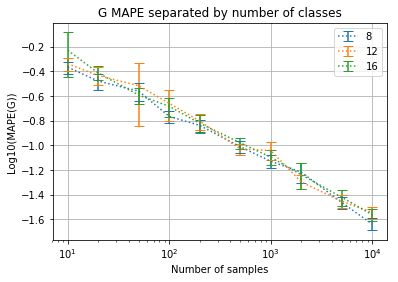
\includegraphics[width=0.45\textwidth]{Chap6_EvaluationAndAnalysis/images/ConvergenceNumberOfClasses_LM.png}
\end{subfigure}
\begin{subfigure}
    \centering
    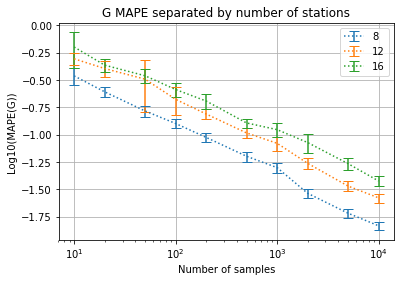
\includegraphics[width=0.45\textwidth]{Chap6_EvaluationAndAnalysis/images/ConvergenceNumberOfStations_LM.png}
\end{subfigure}
\caption{Convergence plot for large models, separated by number of classes and stations.}
\label{fig:ClassSeparatedConvergence_LM}
\end{center}
\end{figure}

The same values are shown in figure \ref{fig:ClassSeparatedConvergence_LM_meanerr} without its 95 \% confidence intervals:

\begin{figure}[!htb]
\begin{center}
\begin{subfigure}
    \centering
    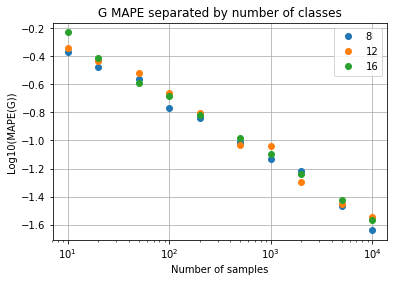
\includegraphics[width=0.45\textwidth]{Chap6_EvaluationAndAnalysis/images/ConvergenceNumberOfClasses_LM_meanerr.png}
\end{subfigure}
\begin{subfigure}
    \centering
    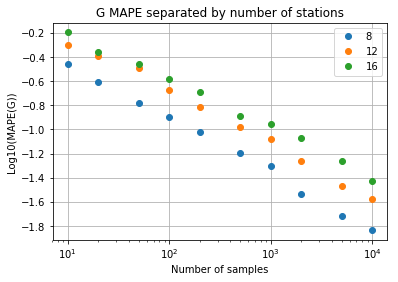
\includegraphics[width=0.45\textwidth]{Chap6_EvaluationAndAnalysis/images/ConvergenceNumberOfStations_LM_meanerr.png}
\end{subfigure}
\caption{Convergence plot for large models, separated by number of classes and stations.}
\label{fig:ClassSeparatedConvergence_LM_meanerr}
\end{center}
\end{figure}

\section{Effects of Transforms and Sampling Distribution}\label{sec:Transforms_and_Distributions}

For this section we analyze the behaviour of the normalizing constant error \(\epsilon\) when integration sampling distribution (gaussian or student-t), and the type of logistic transform (additive or multiplicative) is changed. When performing a comparison, models with the same number of stations and classes are considered in isolation, in order to remove the effect the model size has on the error distribution, since errors can have strong dependence on the model size. This allows us to perform a better analysis of the errors. The (number of station, number of classes) \((K,R)\) pairs tested were : \((2,2), (4,4), (6,6)\)

\subsection{Choice of Sampling Distribution}

For all 3 cases : \((K=R=2)\), \((K=R=4)\), \((K=R=6)\), the results were very similar qualitatively. Here we will present plots and figures for the case \(K=R=6\). Tables for \(K=R=2\) and \(K=R=4\) are provided in appendix \ref{app:extra_experiments}. The transform used was the additive logistic transform.
\\\\
\textit{{\large Multivariate Gaussian Sampling Distribution}}
\\\\
In this comparison, two types of sampling distributions were considered: the Multivariate Gaussian, and the Multivariate Student-t distribution. The shapes of these distributions can approximate the shape of the integrand well by using the Hessian \(\mathbf{A}\) at the stationary point \(\mathbf{\hat{x}}\) as the covariance matrix \(\boldsymbol{\Sigma} = \mathbf{A}^{-1}\).
\\\\
In the case of the Multivariate Gaussian, a slight change was made: a scaling factor \(s\) was introduced to the covariance matrix \(\boldsymbol{\Sigma} = s\mathbf{A}^{-1}\). This allows the multivariate Gaussian to sample from a larger area in the region around the integrand mode. 
\\\\
\begin{figure}[!htb]
\begin{center}
\begin{subfigure}
    \centering
    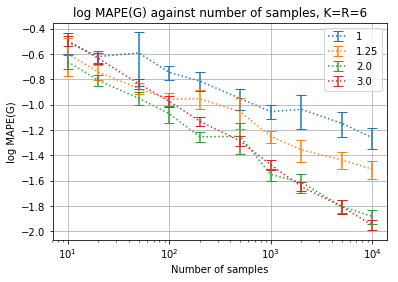
\includegraphics[width=0.45\textwidth]{Chap6_EvaluationAndAnalysis/distribution_variation/Convergence_scale_KR6_gaussian.png}
\end{subfigure}
\begin{subfigure}
    \centering
    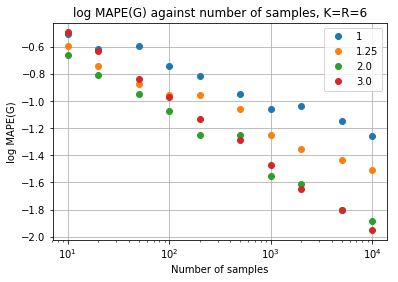
\includegraphics[width=0.45\textwidth]{Chap6_EvaluationAndAnalysis/distribution_variation/Convergence_scale_KR6_gaussian_meanerr.png}
\end{subfigure}
\caption{Convergence plot for \(K=R=6\) models, when integrated using different scales \(s\) for the Gaussian Covariance. On the left is a plot of the log of MAPE , with \(95\%\) confidence intervals. The MAPE estimate is on the right without errorbars}
\label{fig:ConvergencePlotGaussianScales}
\end{center}
\end{figure}

It can be seen in the MAPE convergence plot \ref{fig:ConvergencePlotGaussianScales} that for smaller values of \(s\), the error statistics are more noisy. Besides that, on average, the MAPE values are higher. As \(s\) increases, the plots becomes less noisy, and errors decrease on average. A quick inspection of the error histograms shows why this is the case:

\begin{figure}[!htb]
\begin{center}
    \centering
    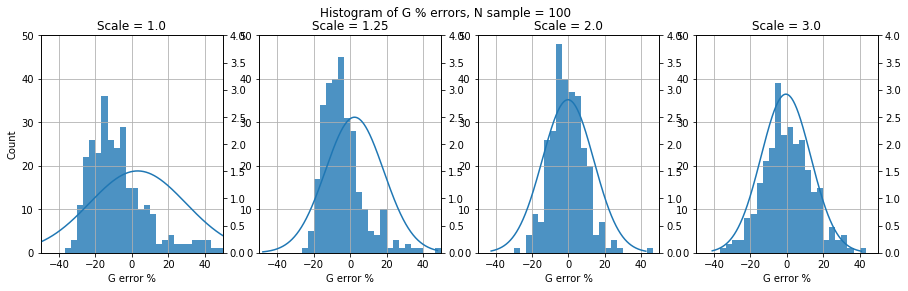
\includegraphics[width=1.0\textwidth]{Chap6_EvaluationAndAnalysis/distribution_variation/hist_KR6_gaussian.png}    
\caption{Error histograms of the errors vs. its Max Likelihood Gaussian for models where \(K=R=6\), and number of samples = \(100\), and different scales \(s\)}
\label{fig:hist_KR6_gaussian}
\end{center}
\end{figure}

\begin{figure}[!htb]
\begin{center}
    \centering
    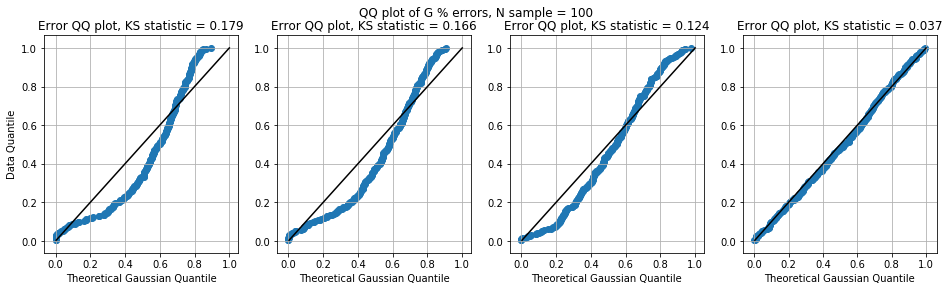
\includegraphics[width=1.0\textwidth]{Chap6_EvaluationAndAnalysis/distribution_variation/QQ_KR6_gaussian.png}
\caption{QQ plot of the errors vs. its Max Likelihood Gaussian for models where \(K=R=6\), and number of samples = \(100\), with different scales \(s\).}
\label{fig:QQ_KR6_gaussian}
\end{center}
\end{figure}

We can observe from figures \ref{fig:hist_KR6_gaussian} and \ref{fig:QQ_KR6_gaussian} that for smaller values of \(s\), not only the error distribution is poorly approximated by a normal distribution, but that the error of \(G\) is negatively biased - i.e. the Logistic Sampling algorithm has a tendency to underestimate the normalizing constant. Besides that, the error distributions for smaller \(s\) have heavier tails, indicating many outliers, which explains the noisiness in the mean error. As \(s\) is increased, the error distribution approaches the normal distribution, and the bias disappears.
\\\\
\textit{{\large Multivariate Student-t Sampling Distribution}}
\\\\
Next the Logistic Sampling algorithm was tested with the student-t distribution as the integration sampling distribution. Similarly to the multivariate Gaussian, the covariance parameter \(\boldsymbol{\Sigma}\) here used was the inverse of the Hessian of the logistic integrand. The experiments here involved changing the degree-of-freedom (DOF) parameter of the t-distribution (denoted \(\nu\)), and observing its error distribution.
\\\\
\begin{figure}[!htb]
\begin{center}
\begin{subfigure}
    \centering
    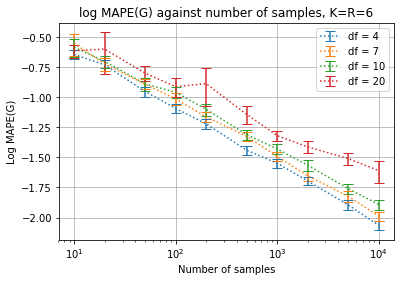
\includegraphics[width=0.45\textwidth]{Chap6_EvaluationAndAnalysis/distribution_variation/Convergence_DF_KR6_tdist.png}
\end{subfigure}
\begin{subfigure}
    \centering
    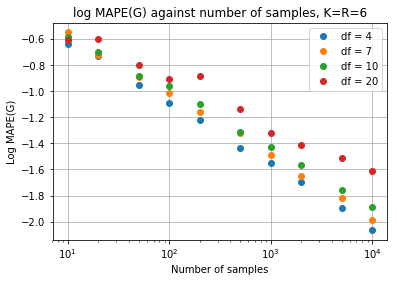
\includegraphics[width=0.45\textwidth]{Chap6_EvaluationAndAnalysis/distribution_variation/Convergence_DF_KR6_tdist_meanerr.png}
\end{subfigure}
\caption{Convergence plot for \(K=R=6\) models, when integrated using different values of the DOF \(\nu\). On the left is a plot of the MAPE, with \(95\%\) confidence intervals, the right without.}
\label{fig:ConvergencePlotTDOF}
\end{center}
\end{figure}

It was observed that varying \(\nu\) had a very similar effect to varying the covariance scale \(s\) in the case of the experiments Multivariate Gaussian sampling distribution. An increase in the value of \(\nu\) has a similar effect to decreasing the value of \(s\). As \(\nu\) is increased, the error distribution becomes more negatively biased and less symmetric, with heavier tails. This naturally makes the approximation \(\bar{M}\) more noisy. This is expected since the student-t sampling distribution approaches the Gaussian sampling distribution with scale \(s=1\), as \(\nu \rightarrow \infty\).

\begin{figure}[!htb]
\begin{center}
    \centering
    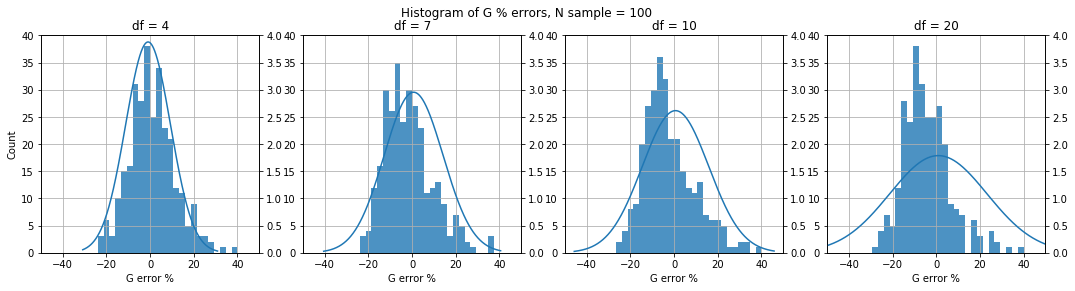
\includegraphics[width=1.0\textwidth]{Chap6_EvaluationAndAnalysis/distribution_variation/hist_KR6_tdist.png}
\caption{Error histograms of the errors vs. its Max Likelihood Gaussian for models where \(K=R=6\), and number of samples = \(100\), and different DOF values \(\nu\)}
\label{fig:hist_KR6_tdist}
\end{center}
\end{figure}

\begin{figure}[!htb]
\begin{center}
    \centering
    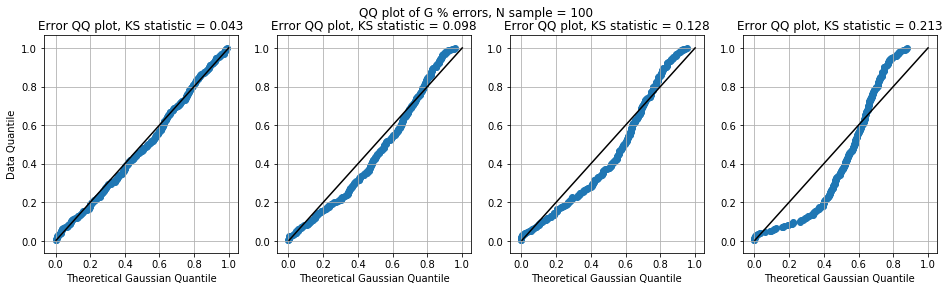
\includegraphics[width=1.0\textwidth]{Chap6_EvaluationAndAnalysis/distribution_variation/QQ_KR6_tdist.png}
\caption{QQ plot of the errors vs. its Max Likelihood Gaussian for models where \(K=R=6\), and number of samples = \(100\), and different DOF values \(\nu\)}
\label{fig:QQ_KR6_tdist}
\end{center}
\end{figure}

\begin{figure}[!htb]
\begin{center}
\begin{subfigure}
    \centering
    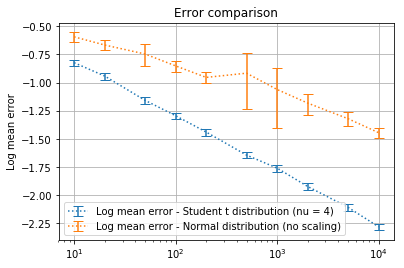
\includegraphics[width=0.45\textwidth]{Chap6_EvaluationAndAnalysis/distribution_variation/Convergence_KR6_tdist_vs_gaussian_s100.png}
\end{subfigure}
\begin{subfigure}
    \centering
    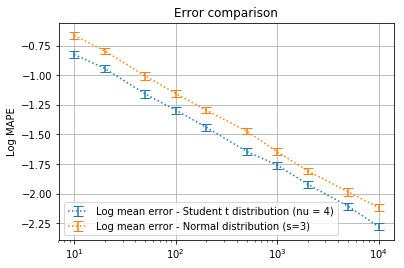
\includegraphics[width=0.45\textwidth]{Chap6_EvaluationAndAnalysis/distribution_variation/Convergence_KR6_tdist_vs_gaussian_s300.png}
\end{subfigure}
\caption{Convergence plot for \(K=R=6\) models. (Left) Comparison of student-t sampling distribution with \(\nu=4\) vs Gaussian sampling distribution with \(s=1\). (Right) Student-t with \(\nu=4\) vs Gaussian with \(s=3\)}
\label{fig:ConvergencePlotTvsGauss}
\end{center}
\end{figure}

A brief visualization of random logistic integrands overlaid with different sampling distributions can help aid understanding in why the sampling distributions play such an important part in reducing variance. Figure \ref{fig:distributiondistribution} shows \(100\) normalized (in both \(x\) and \(y\) axes) logistic integrand functions. The Student-t distribution with \(\nu=4\) and the Gaussian distribution with scale \(s=1\) is overlaid on the plot. The slower decay of the t-distribution away from the stationary point at the centre allows the t-distribution to be more robust in terms of its sampling of important regions in the integrand.
\\\\
As a final choice, the student-t distribution with a degree of freedom of \(\nu=4\) was chosen as the default sampling distribution. The choice for this was motivated by the fact that the t-distribution has some nice mathematical properties, such as a heavier tail that prevents unbounded weights during Monte Carlo sampling (details please refer to section \ref{sec:MCI}). The choice of \(\nu=4\) was supported by the fact that this was the best performing value. Shown below is the standard error comparison between the results from using the t-distribution vs Gaussian distributions.

\begin{figure}[!htb]
\begin{center}
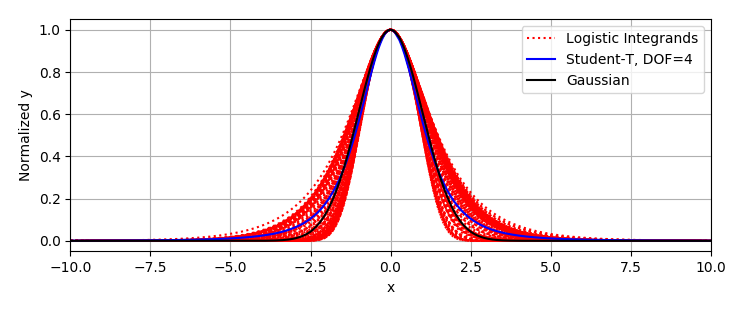
\includegraphics[width=1.\textwidth]{Chap6_EvaluationAndAnalysis/distribution_variation/dist_and_models.png}
\caption{ Randomly generated (2 station) models' logistic functions (normalized in x and y to have unit hessian and \(y=1\) at the stationary point), against a t-distribution (blue) and a Gaussian distribution (black).}
\label{fig:distributiondistribution}
\end{center}
\end{figure}

\subsection{Choice of Transform}

We next turn our attention to the effect of the choice of the logistic transformation on the error distribution. As before, experiments were conducted for the cases: \((K=R=2)\), \((K=R=4)\), and \((K=R=6)\). The conclusions from all 3 studies were very similar, and the version for \((K=R=6)\) is presented here. For plots and tables for the cases \((K=R=2)\), \((K=R=4)\), please refer to appendix \ref{app:extra_experiments}.
\\\\
Shown in table \ref{tab:NC_MAPE_transforms} are the tabulated MAPE (denoted \(\bar{M}(G)\)) and estimated \(95\%\) confidence intervals for the computed normalizing constant. The results for both additive and multiplicative transforms are considered. From a first look, there does not seem to be a significant difference between the two transformations. A more detailed look into the plots and t-distribution of the error prediction confirms this. \\
\begin{table}[!htb]
\begin{center}
    \begin{tabular}{@{}lllllll@{}}
    \toprule
     \(n_s\) & \multicolumn{3}{l}{Additive} & \multicolumn{3}{l}{Multiplicative} \\ \midrule
        & \(\bar{M}(G)\) \% & (-)\% & (+)\% & \(\bar{M}(G)\) \% & (-)\% & (+)\%  \\ \midrule
        10 &\(26.2\) & \(24.4\) & \(28.1\) & \(24.8\) & \(23.1\) & \(26.6\)  \\ 
        20 &\(18.9\) & \(17.8\) & \(20.1\) & \(18.2\) & \(17.2\) & \(19.3\)  \\ 
        50 &\(12.3\) & \(11.6\) & \(12.9\) & \(12\) & \(11.3\) & \(12.7\)  \\ 
        100 &\(8.7\) & \(8.24\) & \(9.16\) & \(8.3\) & \(7.88\) & \(8.71\)  \\ 
        200 &\(6.6\) & \(6.26\) & \(6.94\) & \(6.05\) & \(5.73\) & \(6.37\)  \\ 
        500 &\(4\) & \(3.81\) & \(4.2\) & \(3.75\) & \(3.56\) & \(3.94\)  \\ 
        1000 &\(3.07\) & \(2.93\) & \(3.21\) & \(2.71\) & \(2.57\) & \(2.84\)  \\ 
        2000 &\(2.09\) & \(1.99\) & \(2.19\) & \(1.94\) & \(1.84\) & \(2.04\)  \\ 
        5000 &\(1.22\) & \(1.16\) & \(1.28\) & \(1.18\) & \(1.12\) & \(1.24\)  \\ 
        10000 &\(0.89\) & \(0.846\) & \(0.934\) & \(0.866\) & \(0.821\) & \(0.911\)  \\    \bottomrule
    \end{tabular}
\end{center}
\caption{Normalizing constant MAPE \(M(G)\) \(95 \%\) confidence intervals for \(K=R=6\), for both transforms}
\label{tab:NC_MAPE_transforms}
\end{table}

We first observe the histograms and the quantile-quantile (QQ) plot in figure \ref{fig:ErrorHistAndQQPlot}, and confirm that the error distributions for both transforms are well approximated by a normal distribution.
\begin{figure}[!htb]
\begin{center}
\begin{subfigure}
    \centering
    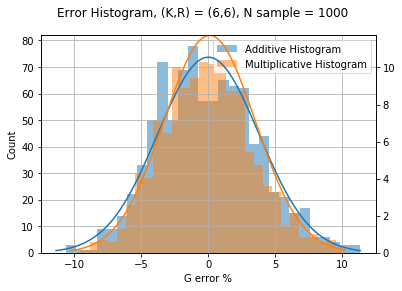
\includegraphics[width=0.45\textwidth]{Chap6_EvaluationAndAnalysis/transform_variation/hist_KR6_transforms.png}
\end{subfigure}
\begin{subfigure}
    \centering
    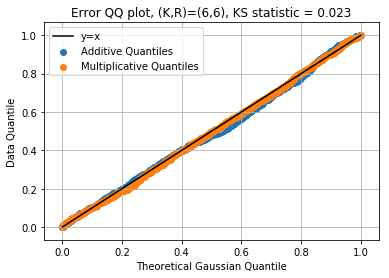
\includegraphics[width=0.45\textwidth]{Chap6_EvaluationAndAnalysis/transform_variation/QQ_KR6_transforms.png}
\end{subfigure}
\caption{(Left) Error distribution histogram and maximum likelihood gaussian. (Right) QQ plot of data quantiles vs. theoretical quantiles. \(N_{sample}=1000\)}
\label{fig:ErrorHistAndQQPlot}
\end{center}
\end{figure}

Plotting the estimated mean absolute error \(\bar{M}\) with its confidence intervals in figure \ref{fig:Convergence_Transforms}, it can be seen that the two transforms are quite similar in terms of errors.

\begin{figure}[!htb]
\begin{center}
\begin{subfigure}
    \centering
    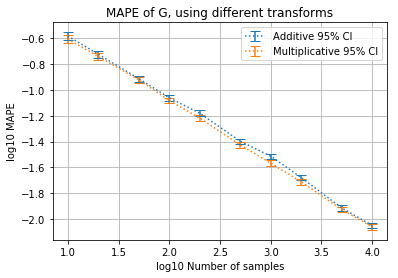
\includegraphics[width=0.45\textwidth]{Chap6_EvaluationAndAnalysis/transform_variation/Stderr_convergence_KR6_transforms.png}
\end{subfigure}
\begin{subfigure}
    \centering
    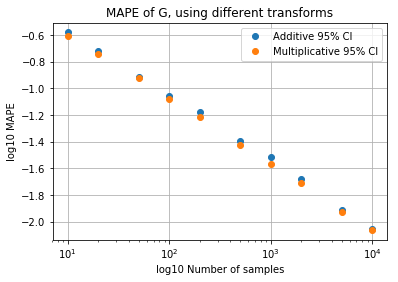
\includegraphics[width=0.45\textwidth]{Chap6_EvaluationAndAnalysis/transform_variation/MAPE_convergence_KR6_transforms.png}
\end{subfigure}
\caption{Convergence plots of MAPE and 95\% confidence intervals from the t-distribution of true MAPE \(M\) (Left), without errorbars (right) for different transforms. }
\label{fig:Convergence_Transforms}
\end{center}
\end{figure}

Figure \ref{fig:Posterior_sigma_transforms} shows the t-distribution estimating the distribution of the true MAPE \(M\). While the t-distributions for the true value of MAPE \(M\) for \(N=100\), \(N=1000\), and \(N=10000\) show a very slight tendency for the multiplicative transform to have a lower MAPE, no conclusive evidence can be drawn due to the large and frequent overlap of the confidence intervals.
\begin{figure}[!htb]
\begin{center}
\begin{subfigure}
    \centering
    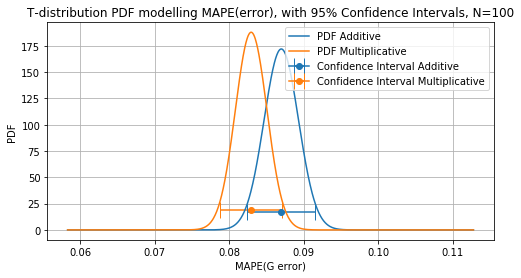
\includegraphics[width=0.45\textwidth]{Chap6_EvaluationAndAnalysis/transform_variation/poterior_KR6_transforms_N100.png}
\end{subfigure}
\begin{subfigure}
    \centering
    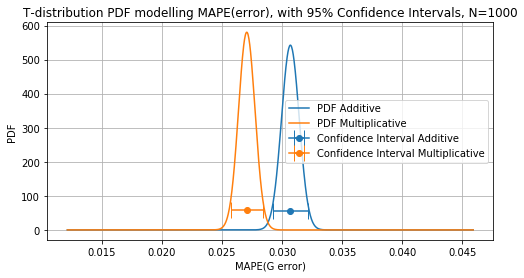
\includegraphics[width=0.45\textwidth]{Chap6_EvaluationAndAnalysis/transform_variation/poterior_KR6_transforms_N1000.png}
\end{subfigure}
\begin{subfigure}
    \centering
    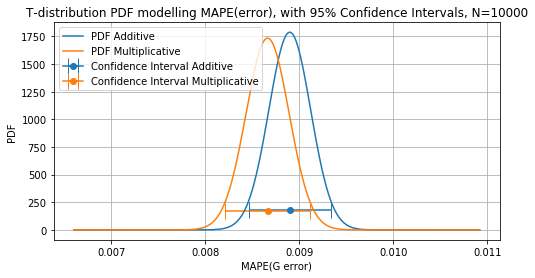
\includegraphics[width=0.45\textwidth]{Chap6_EvaluationAndAnalysis/transform_variation/poterior_KR6_transforms_N10000.png}
\end{subfigure}
\caption{ T - distributions of the true MAPE, given the estimated MAPE \(\bar{M}\) for different transforms.}
\label{fig:Posterior_sigma_transforms}
\end{center}
\end{figure}

From the observed error distributions in this experiments, there is no conclusive evidence to support the fact that one transform has a consistently better performance than the other. 

\section{Introducing Delays}\label{sec:Analyze_Delays}

The introduction of delays into the evaluated model is of interest because it involves evaluating a different integral from from that of the single server case. See sections \ref{sec: multi_server_simplex_integral} and \ref{ssec:infinte_server_networks_results} for details. Table \ref{tab:convergence_tabulated_errors_SM_delay} and figure \ref{fig:OverallConvergence_Delay} shows the convergence behaviour of errors with increasing number of integration samples. This is very similar in terms of trend and magnitudes to that of the single-server case.\\

\begin{table}[!htb] 
\begin{center}
\begin{tabular}{@{}llll@{}}
\toprule
    \(N\) & KS score & \(\bar{M}(G)\)  & \(\hat{\sigma}(G)\) \\  \midrule
    10 &\(0.086\) & \(0.221\) & \(0.332\)  \\ 
    20 &\(0.048\) & \(0.156\) & \(0.206\)  \\ 
    50 &\(0.066\) & \(0.104\) & \(0.144\)  \\ 
    100 &\(0.054\) & \(0.075\) & \(0.100\)  \\ 
    200 &\(0.066\) & \(0.052\) & \(0.077\)  \\ 
    500 &\(0.055\) & \(0.034\) & \(0.046\)  \\ 
    1000 &\(0.056\) & \(0.023\) & \(0.032\)  \\ 
    2000 &\(0.048\) & \(0.017\) & \(0.023\)  \\ 
    5000 &\(0.057\) & \(0.011\) & \(0.014\)  \\ 
    10000 &\(0.033\) & \(0.007\) & \(0.010\)  \\      \bottomrule
\end{tabular}
\end{center}
\caption{Tabulated Mean Absolute Percentage Error, for small models \(K,R \in [2,4,6]\) with delay}
\label{tab:convergence_tabulated_errors_SM_delay}
\end{table} 

\begin{figure}[!htb]
\begin{center}
\begin{subfigure}
    \centering
    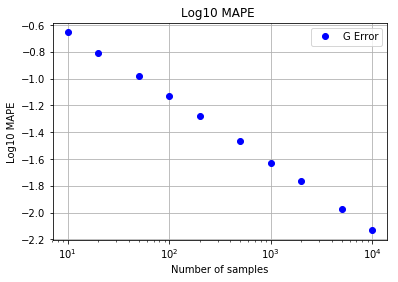
\includegraphics[width=0.45\textwidth]{Chap6_EvaluationAndAnalysis/images/OverallConvergence_Delay.png}
\end{subfigure}
\begin{subfigure}
    \centering
    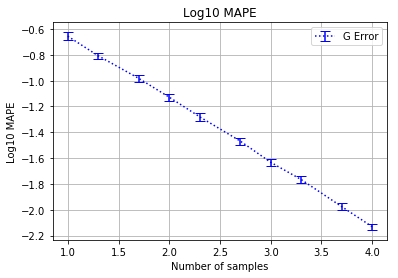
\includegraphics[width=0.45\textwidth]{Chap6_EvaluationAndAnalysis/images/OverallConvergenceSigma_Delay.png}
\end{subfigure}
\caption{ Convergence plots for MAPE \(\bar{M}(G)\) (with 95\% CI's on the right) for small models with delay.}
\label{fig:OverallConvergence_Delay}
\end{center}
\end{figure}

\begin{figure}[!htb]
\begin{center}
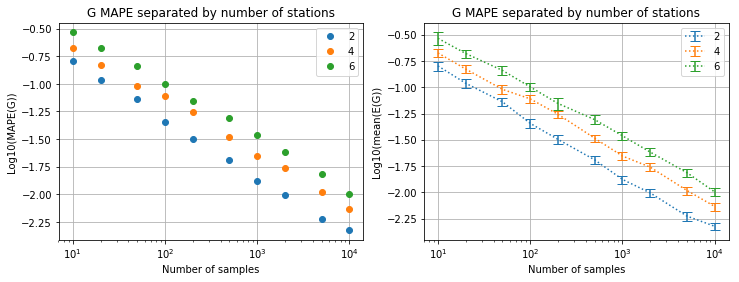
\includegraphics[width=.9\textwidth]{Chap6_EvaluationAndAnalysis/images/ConvergenceNumberOfStations_SM_Delay.png}
\caption{Convergence plots for MAPE \(E(G)\) and standard error \(\sigma\) for small models with delay, separated by number of stations.}
\label{fig:ConvergenceNumberOfStations_SM_Delay}
\end{center}
\end{figure}

Models with delays behave similarly when the number of stations in the network increases. This is shown by the convergence plots in figure \ref{fig:ConvergenceNumberOfStations_SM_Delay}. Finally, comparing the single server only networks alongside the networks with delays, we see that the delay networks have a slightly higher MAPE and standard error. This can be attributed to the fact that an extra dimension is introduced to the integral.

\begin{figure}[!htb]
\begin{center}
\begin{subfigure}
    \centering
    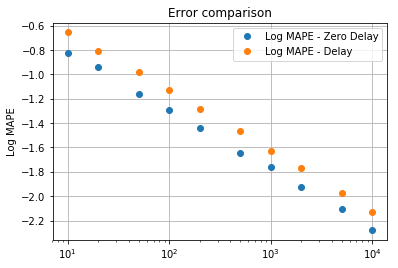
\includegraphics[width=0.45\textwidth]{Chap6_EvaluationAndAnalysis/images/ConvergenceComparison_DelayNoDelay_meanerr.png}
\end{subfigure}
\begin{subfigure}
    \centering
    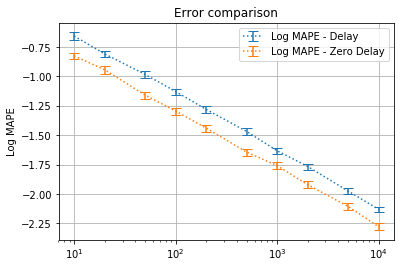
\includegraphics[width=0.45\textwidth]{Chap6_EvaluationAndAnalysis/images/ConvergenceComparison_DelayNoDelay.png}
\end{subfigure}
\caption{ Convergence plots for MAPE \(\bar{M}(G)\) and standard error \(\sigma\) for smalle models with and without delay.}
\label{fig:ConvergenceComparison_DelayNoDelay}
\end{center}
\end{figure}


\section{Multi-server Networks}\label{sec:Multiserver}

\subsection{Variance Cancellation}
In the case of multi-server networks, two approaches to computing the normalizing constant \(\mathbf{G}\) were employed. These were the summations first method, and the integrals first method, summarized in section \ref{sec:Multiserver}. The phenomenon of variance cancellation in the case of integrals first was explained, and in this section, selected experiments are run to demonstrate this phenomenon.
\\\\
In this experiment, a simple 2-station, single class model was considered. The population \(N\) was increased from \(1\) to \(12\). The demand matrix \(\boldsymbol{\theta}\) and the server vector \(\mathbf{s}\) was set as follows:
\[ \boldsymbol{\theta} = \left[ \begin{array}{cc}
0.8 \\
0.6
\end{array} \right]
%
\quad
\mathbf{s} = \left[ \begin{array}{cc}
2 \\
2
\end{array} \right]
\]
Since the normalizing constant is a difference of multiple integrals, we group the positive terms into \(G^{(+)}(\mathbf{x})\) and the negative terms into \(G^{(-)}(\mathbf{x})\):

\begin{equation}
\begin{split}
    G_\theta(\mathbf{N}) & = \frac{1}{\prod_{r=1}^R N_r!} \sum_{\mathbf{0 \leq v <s}} \mathbf{\alpha_v} \boldsymbol{\Delta}_{t_0}^{N-v} \boldsymbol{\Delta}_{\mathbf{t}}^{\mathbf{v}} I(N, t_0, \mathbf{t}) \\
    & = G_\theta^{(+)}(\mathbf{N}) + G_\theta^{(-)}(\mathbf{N})
\end{split}
\end{equation}

Each integral \(I(N, t_0, \mathbf{t})\) was evaluated with \(10^4\) samples. Each model was evaluated 30 times, where the mean value and the standard deviation of \(G_\theta(\mathbf{N})\), \(G_\theta^{(+)}(\mathbf{N})\), and \(G_\theta^{(-)}(\mathbf{N})\) was computed. The results are shown in table \ref{tab:Multiserver_var_cancel}.\\

\begin{table}[!htb] 
\begin{center}
\begin{tabular}{@{}lllllllll@{}}
\toprule
    \(N\) &\(G_{\theta,\text{EXACT}}\) & \(\mu(G^{(+)}_\theta)\) & \(\mu(G^{(-)}_\theta)\)  & \(\mu(G_\theta)\) & \(\sigma(G^{(+)}_\theta)\) & \(\sigma(G^{(-)}_\theta)\)  & \(\sigma(G_\theta)\) \\  \midrule
    1 & \(1.400e+0\) &\(1.400e+0\) & \(0.000e+3\) & \(1.400e+0\) & \(9.283e-4\) & \(0.000e+3\) & \(9.283e-4\) &  \\ 
    2 & \(9.800e-1\) &\(1.972e+0\) & \(-9.917e-1\) & \(9.801e-1\) & \(1.123e-3\) & \(3.937e-4\) & \(1.235e-3\) &  \\ 
    3 & \(5.180e-1\) &\(2.616e+0\) & \(-2.098e+0\) & \(5.181e-1\) & \(1.137e-3\) & \(7.548e-4\) & \(1.332e-3\) &  \\ 
    4 & \(2.450e-1\) &\(3.637e+0\) & \(-3.391e+0\) & \(2.447e-1\) & \(1.340e-3\) & \(1.660e-3\) & \(2.150e-3\) &  \\ 
    5 & \(1.093e-1\) &\(5.132e+0\) & \(-5.023e+0\) & \(1.091e-1\) & \(1.952e-3\) & \(1.725e-3\) & \(2.220e-3\) &  \\ 
    6 & \(4.713e-2\) &\(7.238e+0\) & \(-7.193e+0\) & \(4.854e-2\) & \(2.526e-3\) & \(3.158e-3\) & \(3.796e-3\) &  \\ 
    7 & \(1.987e-2\) &\(1.016e+1\) & \(-1.014e+1\) & \(2.061e-2\) & \(4.119e-3\) & \(3.515e-3\) & \(5.460e-3\) &  \\ 
    8 & \(8.256e-3\) &\(1.421e+1\) & \(-1.420e+1\) & \(9.953e-3\) & \(5.934e-3\) & \(5.881e-3\) & \(8.302e-3\) &  \\ 
    9 & \(3.394e-3\) &\(1.981e+1\) & \(-1.980e+1\) & \(3.656e-3\) & \(6.373e-3\) & \(7.972e-3\) & \(1.064e-2\) &  \\ 
    10 & \(1.385e-3\) &\(2.759e+1\) & \(-2.760e+1\) & \(-3.668e-3\) & \(9.180e-3\) & \(9.310e-3\) & \(1.240e-2\) &  \\ 
    11 & \(5.624e-4\) &\(3.841e+1\) & \(-3.843e+1\) & \(-1.768e-3\) & \(1.784e-2\) & \(1.322e-2\) & \(2.329e-2\) &  \\ 
    12 & \(2.274e-4\) &\(5.346e+1\) & \(-5.349e+1\) & \(-7.763e-3\) & \(2.171e-2\) & \(2.286e-2\) & \(2.850e-2\) &  \\ \bottomrule
\end{tabular}
\end{center}
\caption{Multiserver example variance cancellation}
\label{tab:Multiserver_var_cancel}
\end{table} 

As can be seen in table \ref{tab:Multiserver_var_cancel}, the value of the standard deviation of \(G_\theta\):  \[\sigma(G_\theta) \approx \sqrt{(\sigma(G_\theta^{(+)})^2 + \sigma(G_\theta^{(-)})^2} \]

With small \(N\), this is not a problem since \(\sigma(G_\theta) << G_\theta \approx G_{\theta, \text{EXACT}}\). At about \(N=7\) and \(N=8\), the values of \(G_{\theta}^{(+)}\) and \(G_{\theta}^{(-)}\) become quite large in magnitude, while their respective variances are kept small. However, the magnitude of their differences \(G_\theta\) becomes quite small relative to the standard deviations \(\sigma(G_{\theta}^{(+)})\) and \(\sigma(G_{\theta}^{(-)})\), this can be confirmed by looking at \(G_{\theta,\text{EXACT}}\). Past \(N=8\), the magnitude of the standard deviation is larger than that magnitude of \(G_{\theta,\text{EXACT}}\), and it becomes impossible to recover any information from the approximate solution of \(G_\theta\). 

\subsection{Testing with Fixed Models}

It was eventually agreed that the second method of the multiserver algorithm was to be used. This involves evaluating the following form of the multiserver normalizing constant:
\begin{equation*}
    G_\theta(\mathbf{N}) = \int_{\mathbb{R}^K} \bigg( \frac{1}{\prod_{r=1}^R N_r!} \sum_{\mathbf{0 \leq v <s}} \mathbf{\alpha_v} \boldsymbol{\Delta}_{t_0}^{N-v} \boldsymbol{\Delta}_{\mathbf{t}}^{\mathbf{v}} e^{-h(\mathbf x, t_0, \mathbf{t})}  \bigg) d \mathbf{x}
\end{equation*}

This decision is supported by the following experimental results. 
\\\\
The first test conducted was to perform the same calculations for the model that was used to highlight the variance cancellation phenomenon. The number of samples used was \(n_s=100\), over 2 order of magnitudes less than that used in method 1. For each population \(N\), 100 evaluations were made. The estimated MAPE \(\tilde{M}\), 95\% confidence intervals on the true MAPE \(M\), and the estimated standard error \(\hat{\sigma}_{ML}\) is shown in table \ref{tab:Multiserver_no_var_cancel}. \\

\begin{table}[!htb] 
\begin{center}
\begin{tabular}{@{}llllll@{}}
\toprule
    \(N\) & \(\bar{M} \%\) & \(\bar{M}\) \(95\%\) CI (+) & \(\bar{M}\) \(95\%\) CI (-) & \(\hat{\sigma}_{ML}\)\\ \midrule
    1 &\(0.808\) & \(0.692\) & \(0.924\) & \(0.994\) &  \\ 
    2 &\(0.883\) & \(0.742\) & \(1.02\) & \(1.13\) &  \\ 
    3 &\(0.942\) & \(0.809\) & \(1.08\) & \(1.15\) &  \\ 
    4 &\(0.824\) & \(0.706\) & \(0.943\) & \(1.02\) &  \\ 
    5 &\(0.891\) & \(0.744\) & \(1.04\) & \(1.13\) &  \\ 
    6 &\(0.829\) & \(0.707\) & \(0.952\) & \(1.03\) &  \\ 
    7 &\(0.856\) & \(0.725\) & \(0.986\) & \(1.07\) &  \\ 
    8 &\(0.882\) & \(0.749\) & \(1.01\) & \(1.1\) &  \\ 
    9 &\(0.808\) & \(0.685\) & \(0.93\) & \(1.02\) &  \\ 
    10 &\(1.01\) & \(0.855\) & \(1.17\) & \(1.27\) &  \\ 
    11 &\(1.25\) & \(1.08\) & \(1.42\) & \(1.5\) &  \\ 
    12 &\(1.12\) & \(0.939\) & \(1.31\) & \(1.46\) &  \\  \bottomrule
\end{tabular}
\end{center}
\caption{Multiserver example without variance cancellation}
\label{tab:Multiserver_no_var_cancel}
\end{table}

From table \ref{tab:Multiserver_no_var_cancel}, it can be clearly seen that the evaluated normalizing constants using the second method does not suffer from the same problem as was faced in the first, integrals first method.\\

In a second test, four hand-picked models were tested. We set the number of stations and classes to be \(K=R=2\). In a similar vein to the test with single-server nodes only, we select models which correspond to different loading shares on the stations. This is done by fixing the demand values for station \(0\) to \(1\):
\[\theta_{00} =\theta_{01} = 1\]

Besides that the population vector was fixed to \(\mathbf{N} = [3,3]\). The load shares were varied by changing the demands to station 1, \(\theta_{10}\) and \(\theta_{11}\), as well as the number of servers to stations \(0\) and \(1\), \([s_0, s_1]\). The definition of these models are shown in table \ref{tab:specific_models_evaluate_MS}. For each model, \(300\) evaluations were performed, and the estimated MAPE \(\tilde{M}\) and its confidence intervals were calculated. 
\\\\
The results are shown in table \ref{tab:specific_models_error_MS}. It can be seen that similarly defined models have similar MAPE estimates. The histogram and quantile-quantile plot for the errors for models \(4\) and model \(1\) are shown in figures \ref{fig:multiserver_d0_5s21} and \ref{fig:multiserver_d2s22} respectively. Good conformity with the normal distribution is also observed.

\begin{table}[!htb] 
\begin{center}
\begin{tabular}{@{}lllll@{}}
\toprule
 Test Case &  \([s_0, s_1]\) & \(\theta_{10}, \theta_{11}\) & Description \\ \midrule
 1 & \([2, 2]\) & \(2.0\) & Heavier load on station 1 \\
 2 & \([1, 2]\) & \(2.0\) & Perfectly equal loads\\
 3 & \([2, 2]\) & \(0.5\) & Heavier load on station 0 \\
 4 & \([2, 1]\) & \(0.5\) & Perfectly equal loads \\ \bottomrule
\end{tabular}
\end{center}
\caption{Models tested}
\label{tab:specific_models_evaluate_MS}
\end{table} 

\begin{table}[!htb] 
\begin{center}
\begin{tabular}{@{}llllll@{}}
\toprule
 Test Case & \(\bar{M} \%\) & \(\bar{M}\) \(95\%\) CI (+) & \(\bar{M}\) \(95\%\) CI (-) & \(\hat{\sigma}_{ML}\)\\ \midrule
    1 &\(1.28\) & \(1.17\) & \(1.38\) & \(1.59\) &  \\ 
    2 &\(0.777\) & \(0.71\) & \(0.844\) & \(0.974\) &  \\ 
    3 &\(1.4\) & \(1.27\) & \(1.53\) & \(1.81\) &  \\ 
    4 &\(0.767\) & \(0.703\) & \(0.831\) & \(0.94\) &  \\  \bottomrule
\end{tabular}
\end{center}
\caption{Model errors}
\label{tab:specific_models_error_MS}
\end{table}
 
\begin{figure}[!htb]
\begin{center}
\includegraphics[width=0.8\textwidth]{Chap6_EvaluationAndAnalysis/multiserver/d0_5s21.png}
\caption{ Histogram and QQ plot for model with \(\theta_{10} = \theta_{11} = 0.5\) and \([s_0, s_1] = [2,1]\)}
\label{fig:multiserver_d0_5s21}
\end{center}
\end{figure}

\begin{figure}[!htb]
\begin{center}
\includegraphics[width=0.8\textwidth]{Chap6_EvaluationAndAnalysis/multiserver/d2s22.png}
\caption{ Histogram and QQ plot for model with \(\theta_{10} = \theta_{11} = 0.5\) and \([s_0, s_1] = [2,2]\)}
\label{fig:multiserver_d2s22}\end{center}
\end{figure}

\subsection{Experimentation with Random Single Class Models}
To test the multi-server algorithm with larger models, the following test was carried out:
\begin{itemize}[noitemsep]
    \item Number of classes \(R\) was set to be one
    \item Number of stations was varied, \(K \in [2,4,6]\)
    \item Population \(N\) was chosen to be in \(\mathcal{U}(1,5)\).
    \item Demands were randomized.
    \item The Queue Lengths \(Q_{kr}\) and Throughputs \(\lambda_{r}\) were calculated using the Multiserver Logistic Sampling Algorithm.
    \item The exact queue lengths and throughputs were calculated using the exact MVA algorithm in JMVA. Only single classes are accomodated by the JMVA implementation, hence the restriction on \(R=1\).
\end{itemize}

To calculated the mean queue length per station, the following was used:
\begin{equation*}
    Q_{kr} = \sum_{n_r = 0}^{N_r} n_r P(n_{kr}=n_r | \mathbf{N});
\end{equation*}
Where the marginal probability \(P(n_{kr}=n_r | \mathbf{N})\) was calculated according to:
\begin{equation*}
    P(n_{kr}=n_r | \mathbf{N}) = \sum_{\substack{\mathbf{n}_k \\ n_{kr} = n_r}} F_{k}(\mathbf{n}_k) \frac{ G(-\mathbf{1}_k, \mathbf{N} - \mathbf{n}_k) }{ G(\mathbf{N}) }
\end{equation*}

Where:
\begin{equation*}
\begin{split}
    F_{k}(\mathbf{n}_k) = \frac{1}{\beta(n_k)} n_k! \prod_{r=1}^R \frac{\theta_{kr}^{n_kr}}{n_{kr}!} \\
    \beta(n_k) = \begin{cases} m_k! m_k^{n_k-m_k} & n_k > m_k \\ n_k! & n_k \leq m_k \end{cases}
\end{split}
\end{equation*}

The reported errors are as below:

\begin{table}[!htb] 
\begin{center}
\begin{tabular}{@{}llll@{}}
\toprule
    \(n_s\) & \(Q_{kr}\) MAPE \(\%\) & \(\lambda_r\) MAPE \(\%\) &  \\  \midrule
    10 &\(15.6\) & \(18.8\) &  \\ 
    20 &\(12.3\) & \(13.5\) &  \\ 
    50 &\(8.17\) & \(8.05\) &  \\ 
    100 &\(6.69\) & \(6.13\) &  \\ 
    200 &\(5.1\) & \(4.34\) &  \\ 
    500 &\(3.6\) & \(2.48\) &  \\ 
    1000 &\(3.11\) & \(1.68\) &  \\ 
    2000 &\(2.68\) & \(1.33\) &  \\ 
    5000 &\(2.26\) & \(0.764\) &  \\ 
    10000 &\(2.11\) & \(0.575\) &  \\  \bottomrule
\end{tabular}
\end{center}
\caption{Model errors}
\label{tab:convergence_error_MS}
\end{table}

And the resulting convergence plots are as shown in figure \ref{fig:Convergence_multiserver}.

\begin{figure}[!htb]
\begin{center}
\begin{subfigure}
    \centering
    \includegraphics[width=0.45\textwidth]{Chap6_EvaluationAndAnalysis/multiserver/convergence_MS.png}
\end{subfigure}
\begin{subfigure}
    \centering
    \includegraphics[width=0.45\textwidth]{Chap6_EvaluationAndAnalysis/multiserver/convergence_MS_meanerr.png}
\end{subfigure}
\caption{ Convergence plots for MAPE \(\bar{M}(Q_{kr})\), when compared to exact MVA}
\label{fig:Convergence_multiserver}
\end{center}
\end{figure}

The reason for the unusual trend in the queue length plot is due to the fact that the exact MVA solver reports the queue lengths in the wrong order under certain conditions, which is outside of the scope of this project to debug. Shown in figure \ref{fig:Histogram_multiserver} is the histogram for queue length errors when \(10^3\) and \(10^4\) samples are used. Highlighted are the errors for when the MVA solver reports the queue lengths in the wrong order. The vast majority of queue lengths reported have much lower errors.

\begin{figure}[!htb]
\begin{center}
\begin{subfigure}
    \centering
    \includegraphics[width=0.45\textwidth]{Chap6_EvaluationAndAnalysis/multiserver/histogram_QL_1000samples.png}
\end{subfigure}
\begin{subfigure}
    \centering
    \includegraphics[width=0.45\textwidth]{Chap6_EvaluationAndAnalysis/multiserver/histogram_QL_10000samples.png}
\end{subfigure}
\caption{ Histogram for QL errors (left) when \(10^3\) samples are used, (right) when \(10^4\) samples are used}
\label{fig:Histogram_multiserver}
\end{center}
\end{figure}

\subsection{Experimentation with Random MultiClass Models}
To test the multi-server algorithm with multiclass models, the following test was carried out:
\begin{itemize}[noitemsep]
    \item Number of classes \(R\) was set to be in \([1,2]\)
    \item Number of stations was varied, \(K \in [2,3]\)
    \item Population \(\mathbf{N}\) was chosen to be in \(\mathcal{U}(1,5)\).
    \item Demands were randomized.
    \item The Normalizing Constant \(G_{\boldsymbol{\theta}(\mathbf{N})}\) calculated using the Multiserver Logistic Sampling Algorithm.
    \item The exact answer is calculated using a MATLAB implementation of a recursive algorithm for \(G_{\boldsymbol{\theta}(\mathbf{N})}\) - \texttt{pfqn\_gmvald()}.
\end{itemize}

The model size hyperparameters \(K\), \(R\) and \(N\) were chosen such that the computation times for exact MVA stayed within reasonable limits. The convergence plot is shown in figure \ref{fig:Convergence_NC_multiserver}.

\begin{figure}[!htb]
\begin{center}
\begin{subfigure}
    \centering
    \includegraphics[width=0.45\textwidth]{Chap6_EvaluationAndAnalysis/multiserver/convergence_NC_MS.png}
\end{subfigure}
\begin{subfigure}
    \centering
    \includegraphics[width=0.45\textwidth]{Chap6_EvaluationAndAnalysis/multiserver/convergence_NC_MS_meanerr.png}
\end{subfigure}
\caption{ Convergence plots for MAPE \(\bar{M}(Q_{kr})\), when compared to exact MVA}
\label{fig:Convergence_NC_multiserver}
\end{center}
\end{figure}

The effect of station number on the accuracy is also very similar to the single-server only network case.

\begin{figure}[!htb]
\begin{center}
\includegraphics[width=\textwidth]{Chap6_EvaluationAndAnalysis/multiserver/convergence_NC_MS_meanerr_class_separated.png}
\caption{ Convergence plots for MAPE \(\bar{M}(G)\), when compared to exact MVA}
\label{fig:Convergence_NC_multiserver_class_separated}
\end{center}
\end{figure}

\begin{table}[!htb] 
\begin{center}
\begin{tabular}{@{}lllll@{}}
\toprule
    \(n_s\) & \(95\% (+)\) \(\%\) & \(95\% (-)\) \(\%\) & \(\bar{M} \%\) &  \\  \midrule
    10 &\(7.47\) & \(6.27\) & \(6.87\) &  \\ 
    20 &\(5.26\) & \(4.28\) & \(4.77\) &  \\ 
    50 &\(3.23\) & \(2.69\) & \(2.96\) &  \\ 
    100 &\(2.25\) & \(1.87\) & \(2.06\) &  \\ 
    200 &\(1.7\) & \(1.4\) & \(1.55\) &  \\ 
    500 &\(0.972\) & \(0.801\) & \(0.886\) &  \\ 
    1000 &\(0.727\) & \(0.601\) & \(0.664\) &  \\ 
    2000 &\(0.543\) & \(0.445\) & \(0.494\) &  \\ 
    5000 &\(0.333\) & \(0.277\) & \(0.305\) &  \\ 
    10000 &\(0.244\) & \(0.203\) & \(0.224\) &  \\  \bottomrule
\end{tabular}
\end{center}
\caption{Tabulated MAPE for the computation of the normalizing constant, with \(95\%\) confidence intervals}
\label{tab:convergence_error_MS_NC}
\end{table}


\subsection{A few notes on large models}
It was observed that under larger models (large \(K\), \(R\) or \(N\)), the stationary point search can yield failure. This is due to insufficient precision in the calculation of the integrand, resulting in incorrect integrand values. The solver now takes in a \texttt{precision} argument, which dictates the precision (number of bits) the \texttt{BigDecimal} operations in the Logistic Sampling Algorithm uses. A value of \(128\) is sufficient for most small models, otherwise a value of \(256\) can accomodate many large models of interest (eg. \(K,R = 4, N=30 \)).